\documentclass{beamer}
\addtobeamertemplate{navigation symbols}{}{%
\usebeamerfont{footline}%
\usebeamercolor[fg]{footline}%
\hspace{5em}%
\large\insertframenumber
}
\setbeamercolor{footline}{fg=blue}
%\usetheme{Warsaw}

\usepackage[english, russian]{babel}
\usepackage[absolute,overlay]{textpos}

\usefonttheme{professionalfonts}
\usepackage{fontspec}
\setmainfont{Times New Roman}
\setsansfont{Times New Roman}
\setmonofont{Consolas}

\usepackage{tcolorbox}
\usepackage{amsmath}
\usepackage{tikz}
\usepackage{blkarray}
\usepackage{listings}
\lstset{basicstyle=\footnotesize\ttfamily}
\lstset{escapeinside={<@}{@>}}
\usepackage[cache=false]{minted}
\newminted{python}{fontsize=\scriptsize, linenos=false}

\graphicspath{{../images/}}

\title{Моделирование перераспределения потоков между трещинами гидроразрыва пласта}
\subtitle{}
\author{Выполнил студент: А.~А.~Муравцев\and \\Научный руководитель: С.~А.~Калинин\and \\Консультант: И.~Ш.~Базыров}

%\institute{
%\inst{1}
%Высшая школа теоретической механики и математической физики\\
%Санкт-Петербургский Политехнический университет Петра Великого
%}

\definecolor{new_green}{rgb}{0.20,0.68,0}
\definecolor{lit_gray}{gray}{0.3}

\begin{document}


\begin{frame}
\titlepage
\end{frame}


\begin{frame}
\frametitle{Проблематика и актуальность работы}
\begin{itemize}
	\item при эксплуатации месторождения во время перевода скважин с проведённым многостадийным гидроразрывом пласта в нагнетание (с целью поддержания пластового давления) практически невозможно избежать роста нескольких трещин автоГРП
	%\item при прорыве трещин автоГРП к добывающим скважинам существенно снижаются площадь охвата заводнением и эффективность эксплуатации месторождения
	\item важно научиться моделировать одновременный рост нескольких трещин автоГРП и перераспределение потоков между ними, чтобы не допускать снижение эффективности эксплуатации месторождения вследствие прорыва трещин автоГРП к добывающим скважинам 
\end{itemize}
\end{frame}


\begin{frame}
\frametitle{Цель и задачи работы}

\textbf{Цель:}
\begin{itemize}
	\item построить модель совместного роста нескольких трещин автоГРП с учётом перераспределения потоков между ними
\end{itemize}

\textbf{Задачи:}
\begin{itemize}
	\item провести обзор имеющихся моделей роста трещины гидроразрыва пласта и выбрать наиболее подходящую модель для роста трещины автоГРП
	\item построить физико-математическую модель роста нескольких трещин автоГРП
	\item реализовать численный алгоритм решения на Python
	\item построить графики зависимостей полудлины каждой из трещин автоГРП и расходов на каждой из трещин от времени
	\item построить график зависимости забойного давления от времени
\end{itemize}

\end{frame}


\begin{frame}
\frametitle{Основные компоненты полной модели трещины ГРП}

\begin{textblock*}{8.8cm}(0.5cm,1.5cm)
\begin{enumerate}[1)]
	\item закон сохранения жидкости (доминирование или отсутствие утечек);
	\item уравнение течения жидкости в трещине (в зависимости от реологии жидкости);
	\item уравнение упругости для горной породы;
	\item условие распространения трещины;
	\item транспорт проппанта
\end{enumerate}
\end{textblock*}

\begin{textblock*}{3cm}(9.5cm,1.5cm)
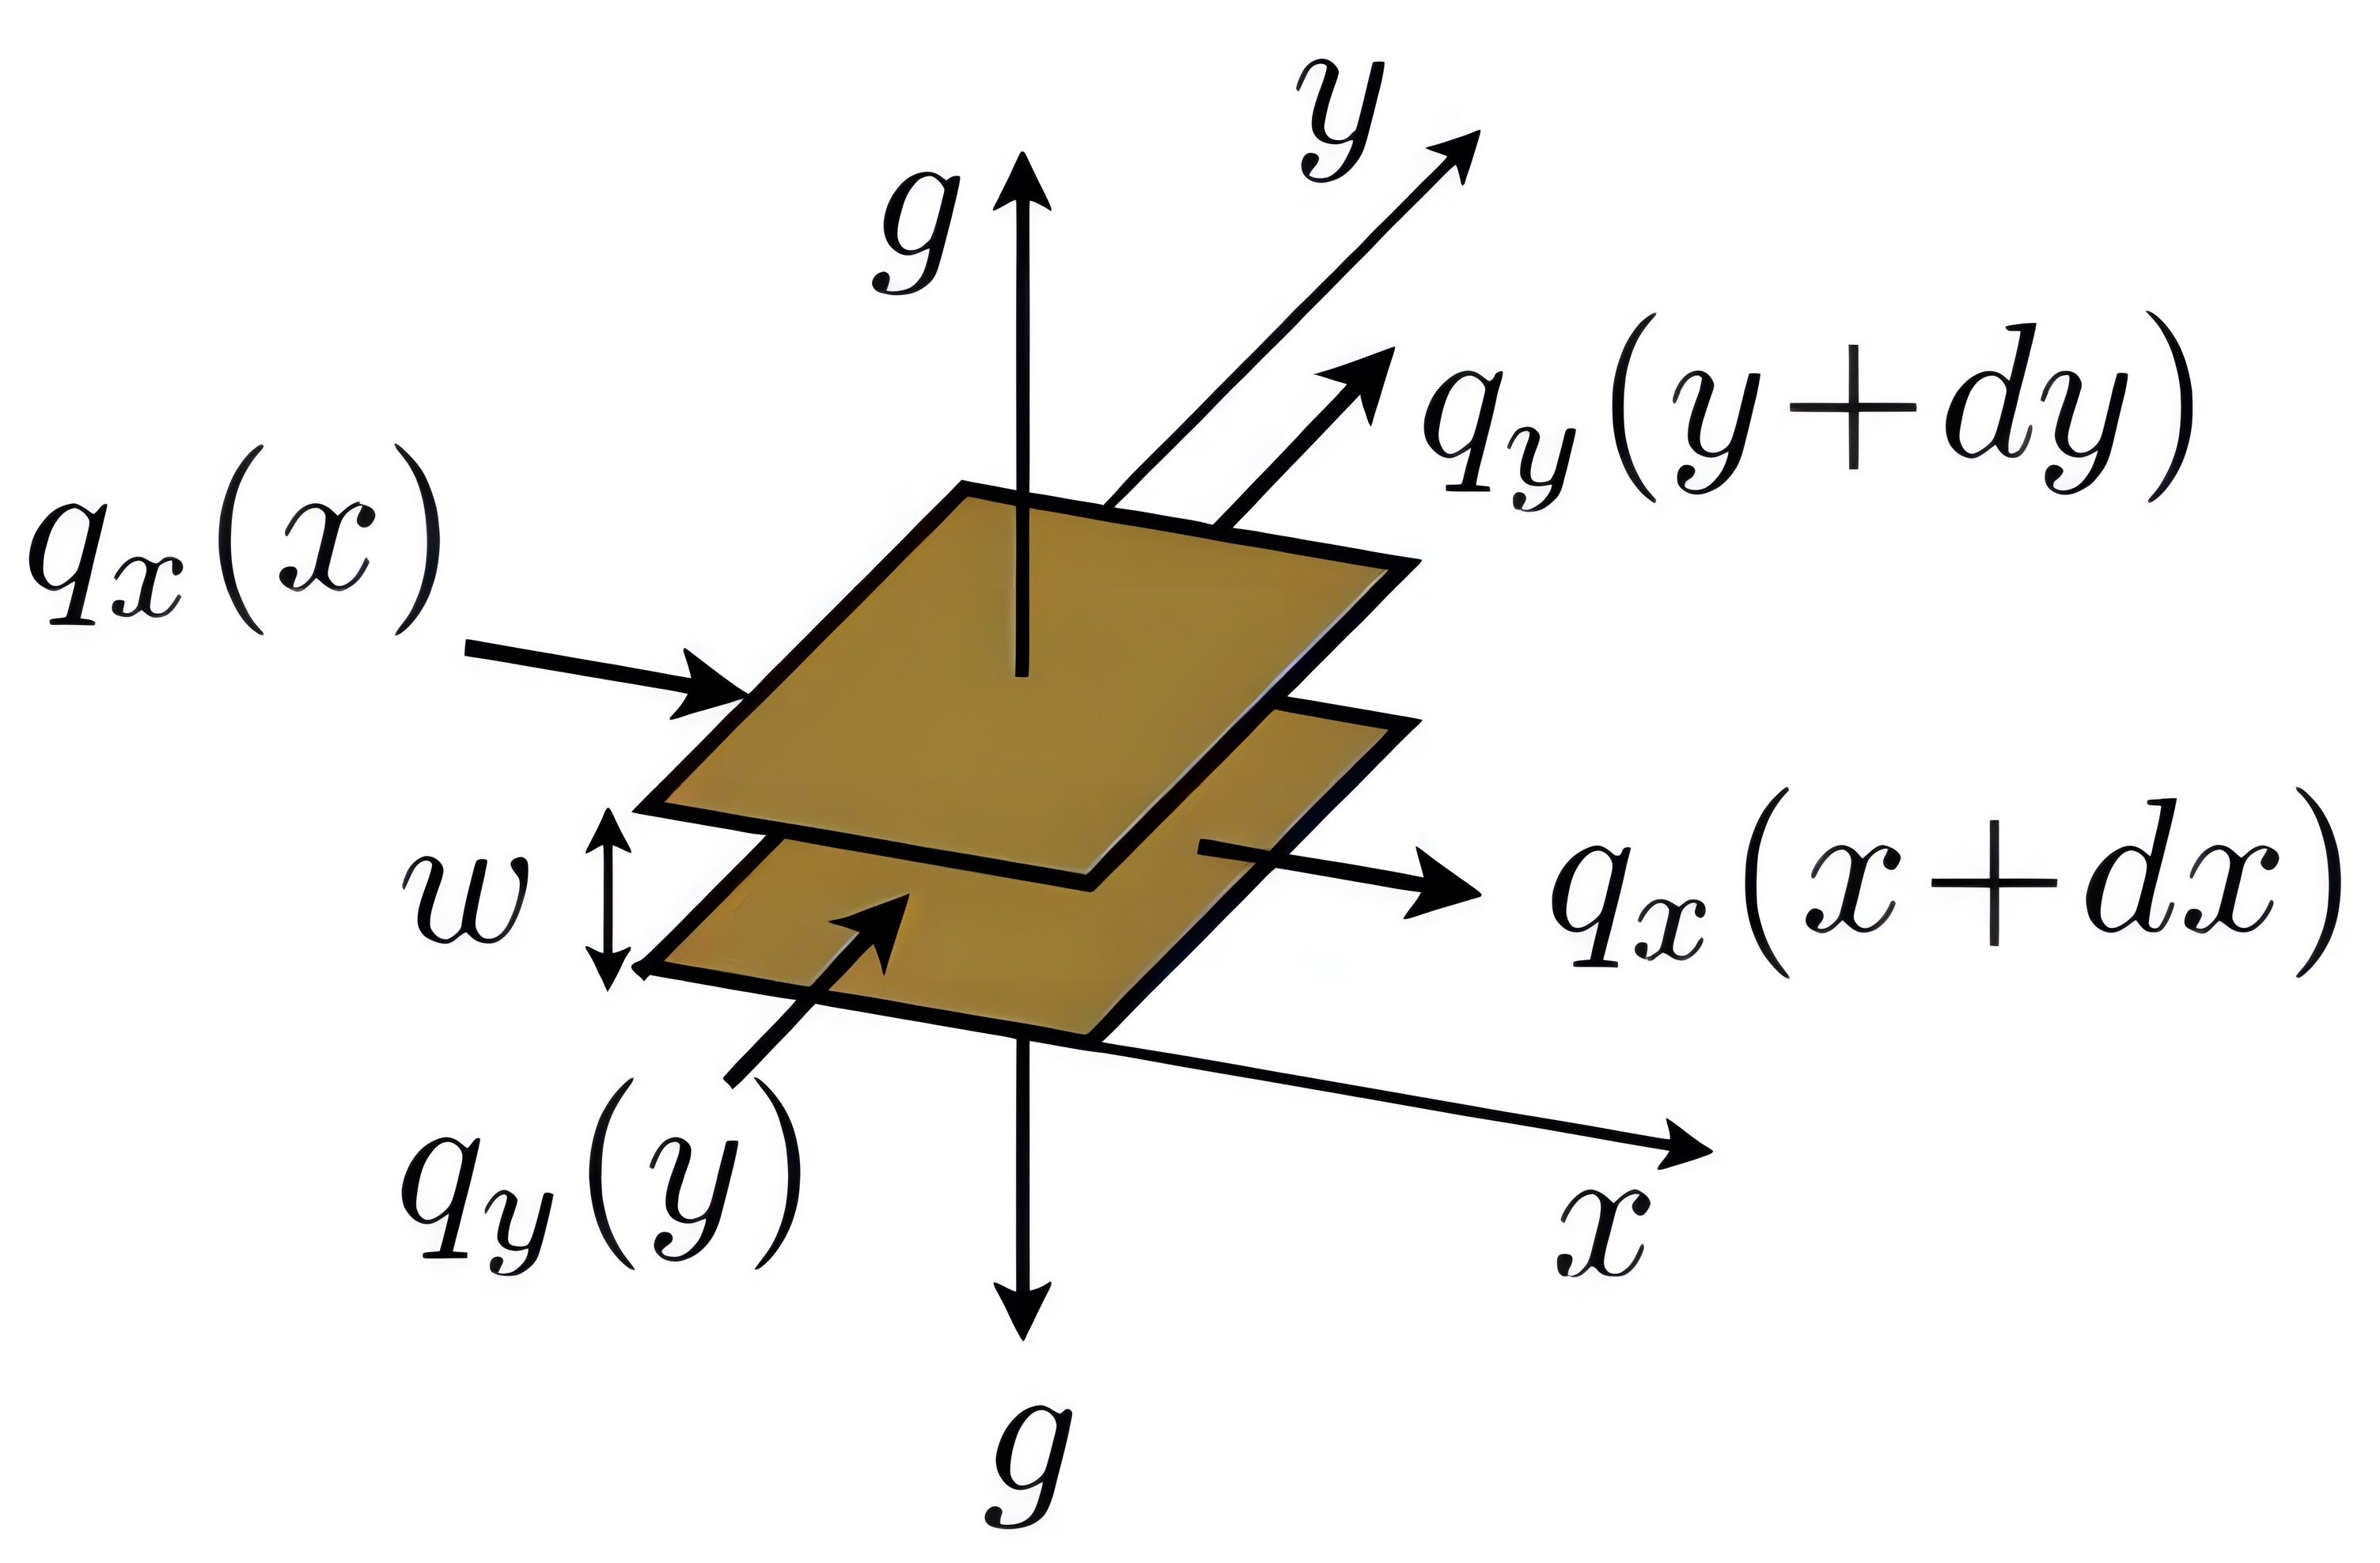
\includegraphics[width=3cm]{part1_balance.jpg}
\end{textblock*}

\begin{textblock*}{4cm}(0.5cm,6cm)
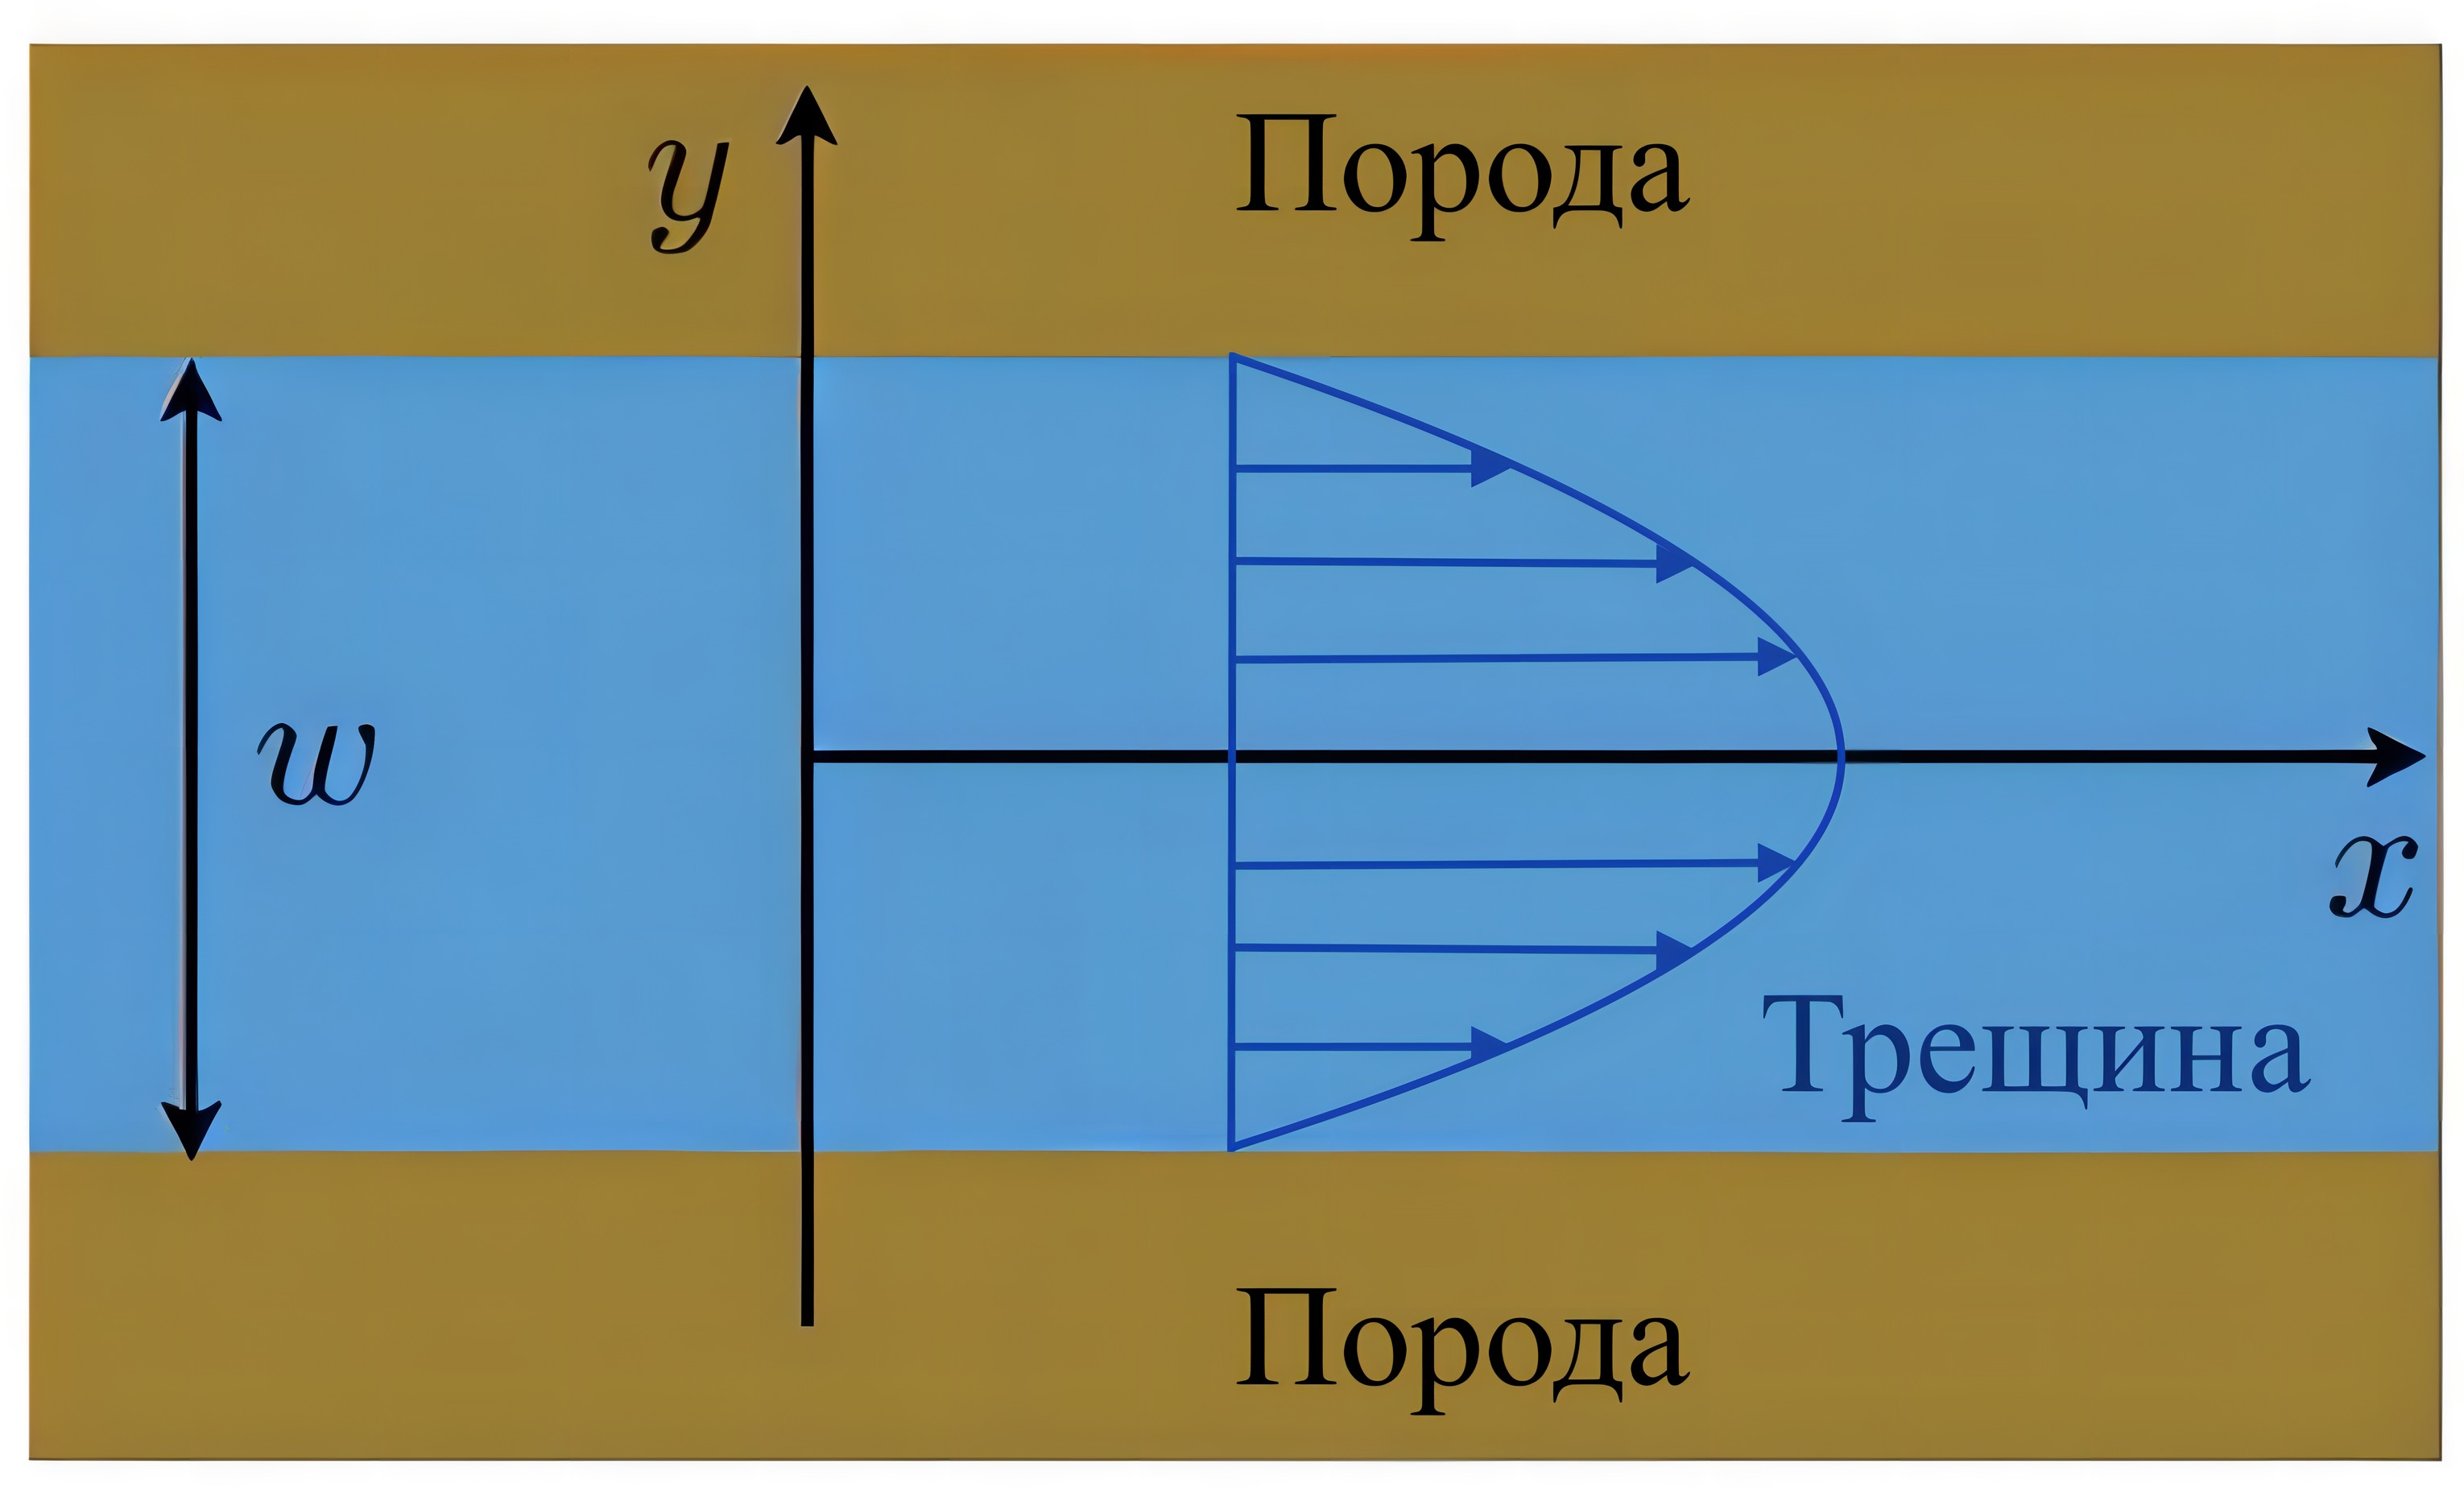
\includegraphics[width=4cm]{part2_flux.jpg}
\end{textblock*}

\begin{textblock*}{3.5cm}(8.5cm,3.7cm)
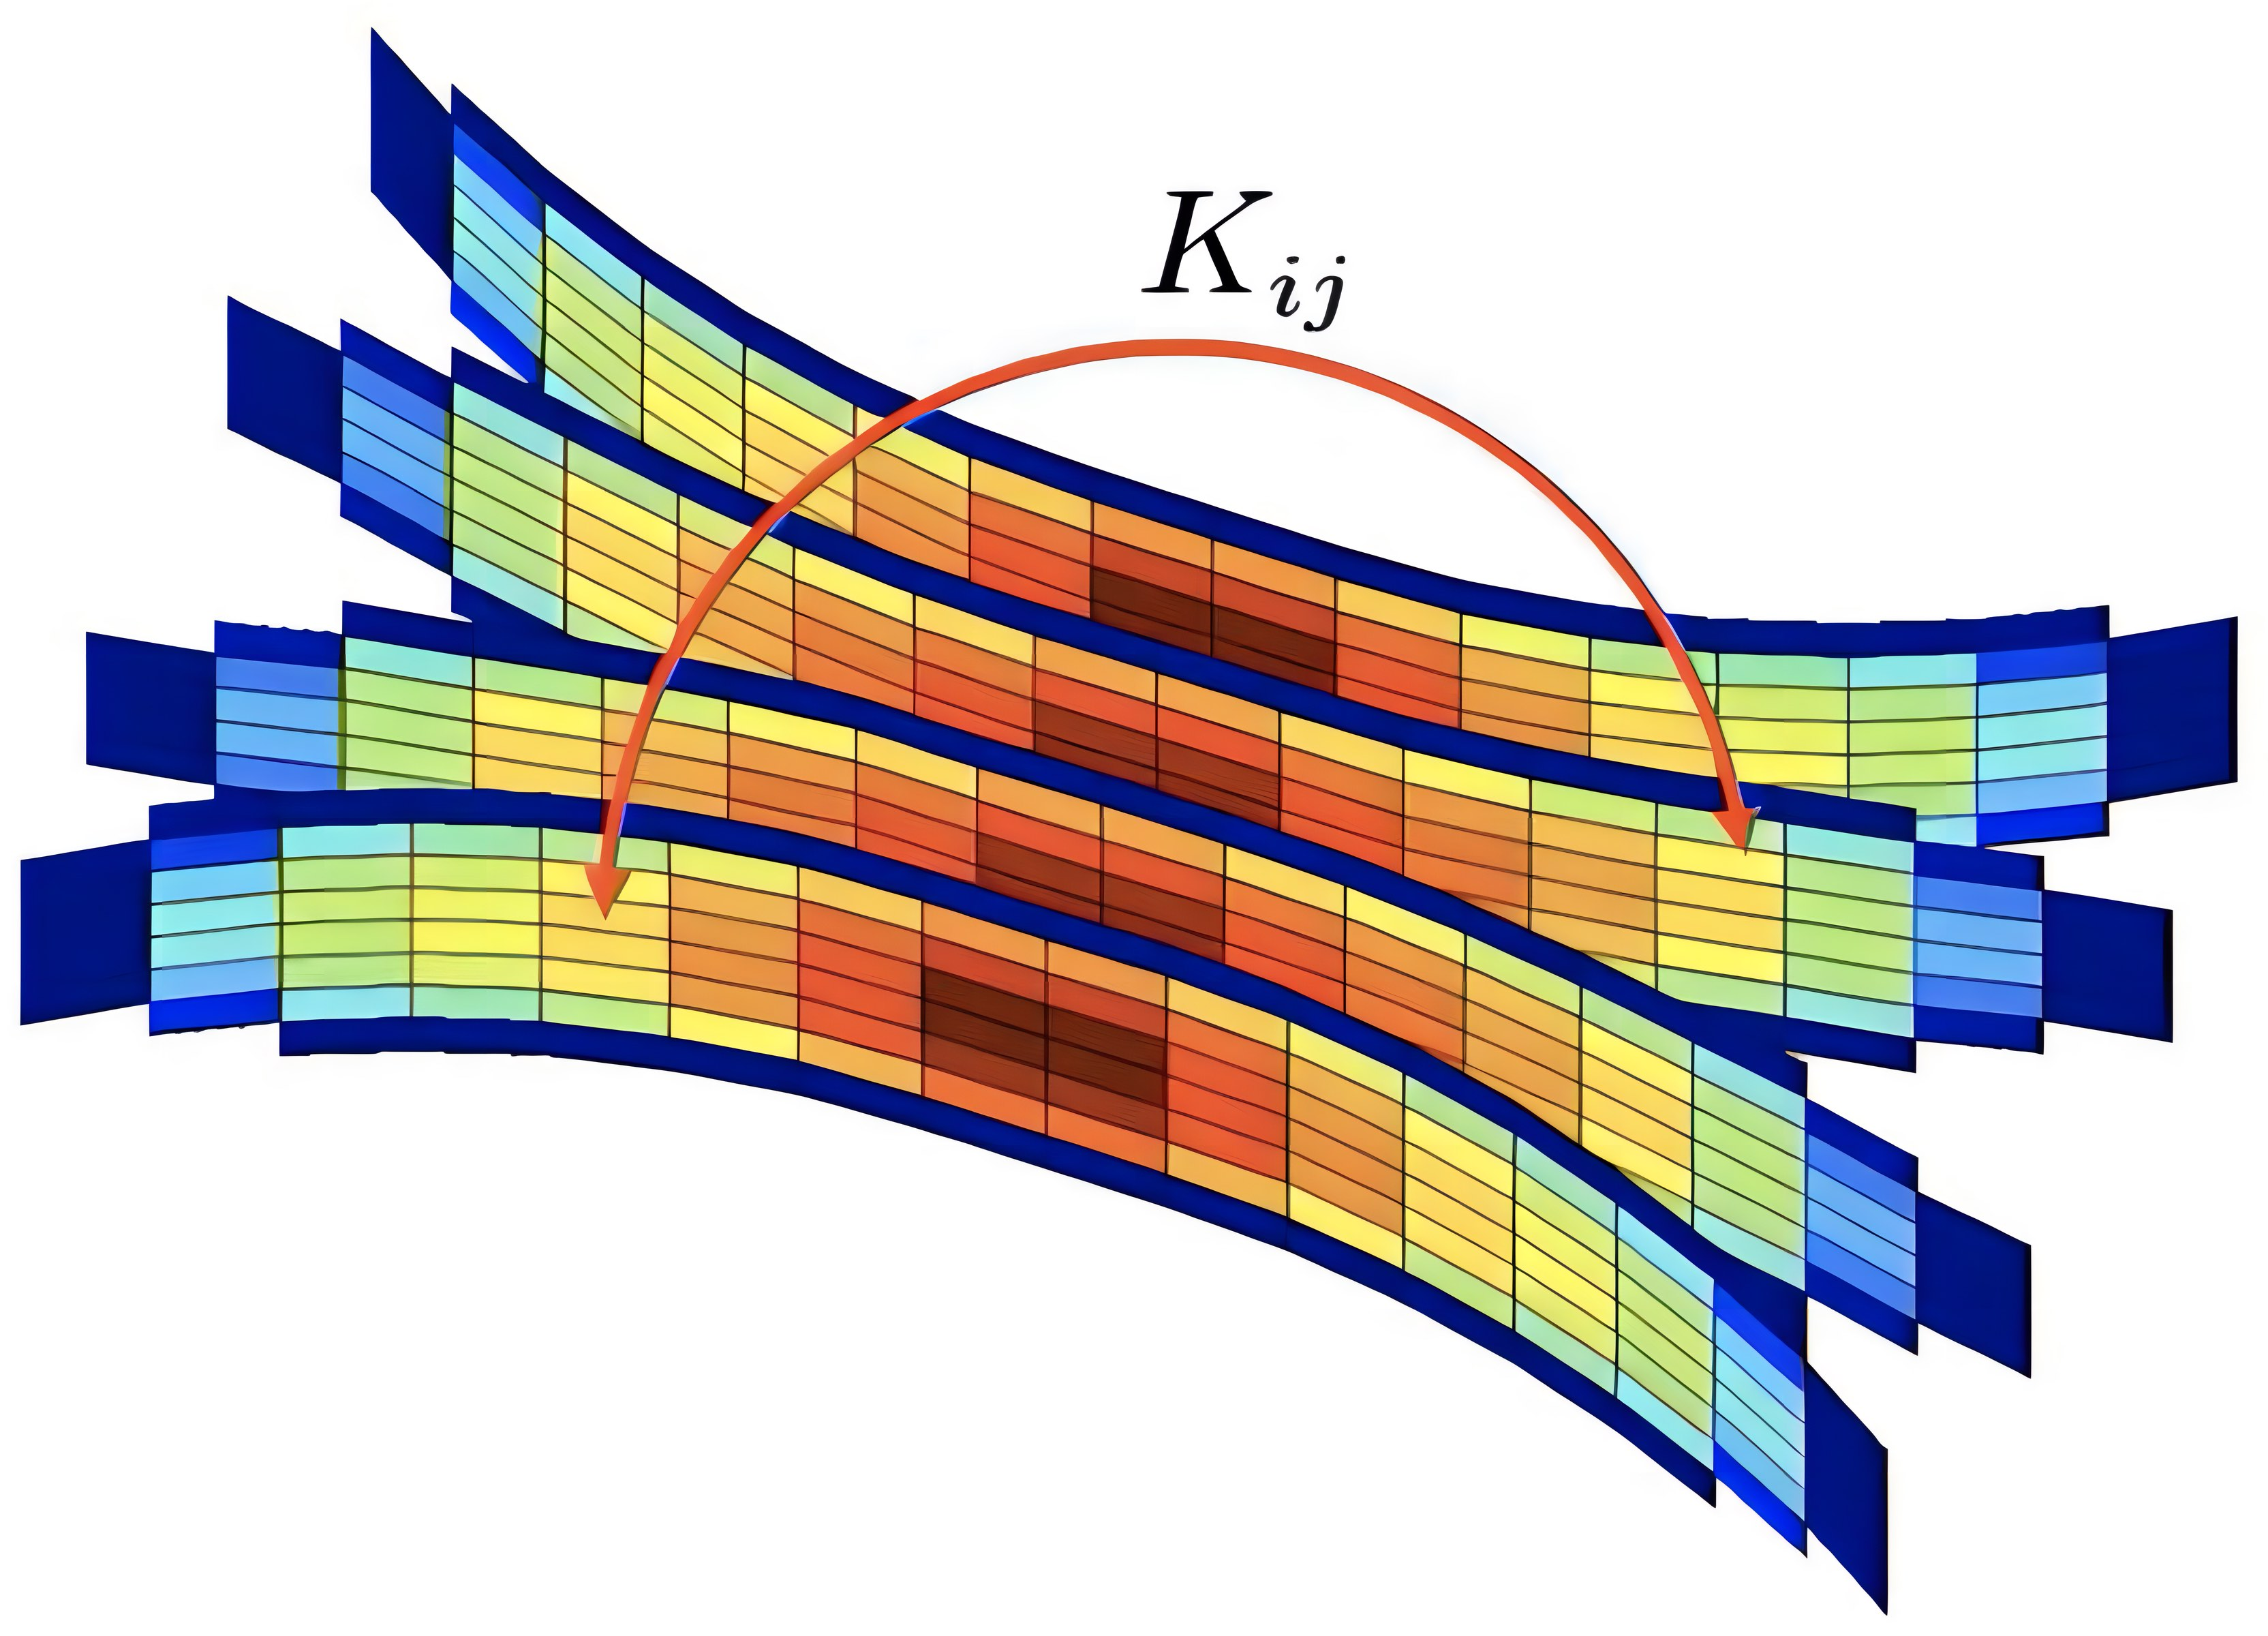
\includegraphics[width=3.5cm]{part3_elasticity.jpg}
\end{textblock*}


\begin{textblock*}{3cm}(5.5cm,5.3cm)
\tiny
$$
w=\sqrt{\frac{32}{\pi}}\frac{K_{I}\left(1-\nu^2\right)}{E}\sqrt{r}
$$
\normalsize
\end{textblock*}

\begin{textblock*}{7.5cm}(5cm,6.5cm)
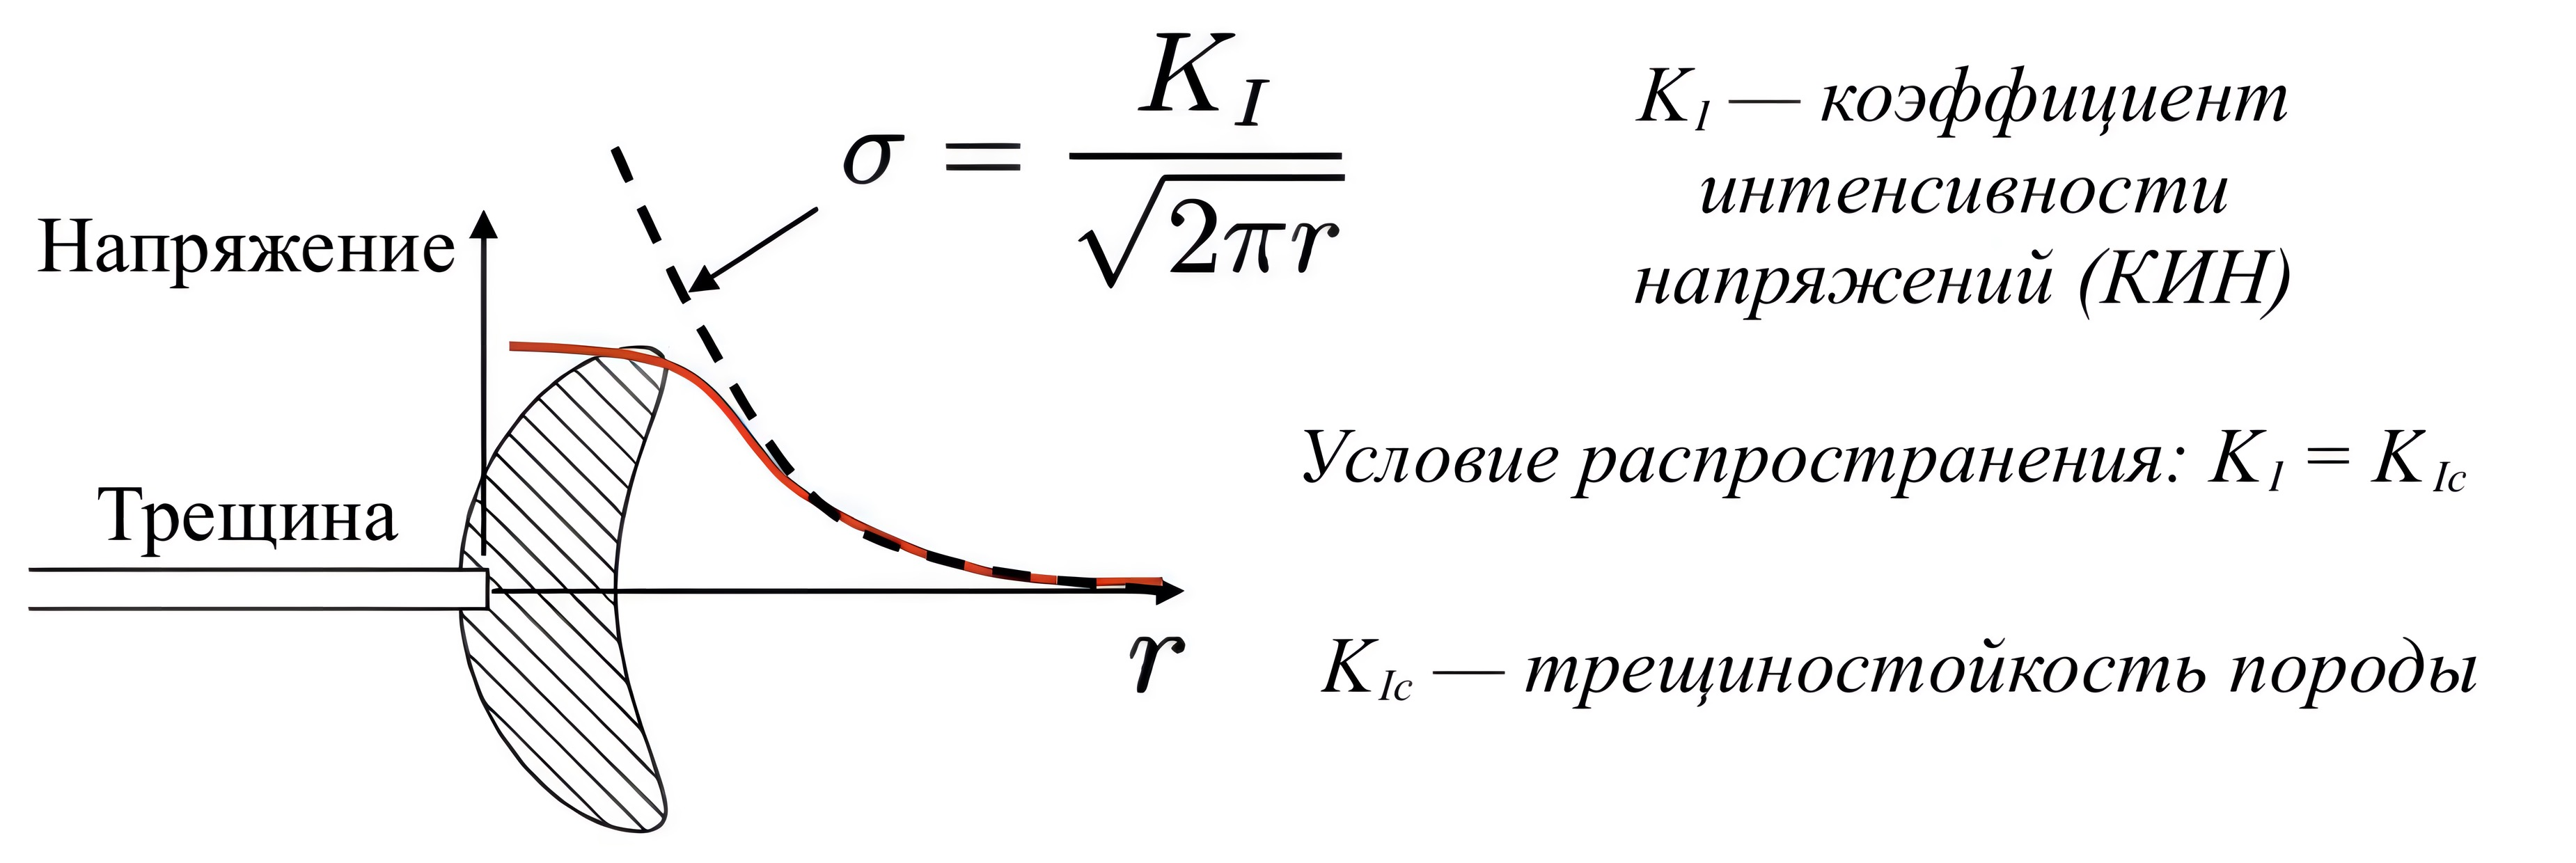
\includegraphics[width=7.5cm]{part4_propagation.jpg}
\end{textblock*}

\begin{textblock*}{6cm}(0.5cm,8.9cm)
\tiny
\textcolor{lit_gray}{J.R. Rice. Mathematical analysis in the mechanics of fracture. Fracture: an advanced treatise, vol. II, pp. 191-311, 1968}
\end{textblock*}

\end{frame}


\begin{frame}
\frametitle{Модель Христиановича-Желтова-Гиртсма-деКлерка (модель плоской трещины)}

\footnotesize

\begin{textblock*}{6cm}(0.5cm,1.7cm)
$$
\begin{cases}
\dfrac{\partial w}{\partial t}+\dfrac{\partial q}{\partial x}+\dfrac{C'}{\sqrt{t-t_0(x)}}=Q_0(t)\delta(x),\\[15pt]
q=-\dfrac{w^3}{\mu'}\dfrac{\partial p}{\partial x},\\[5pt]
p(x,t)=\sigma_0-\dfrac{E'}{4\pi}\displaystyle\int\limits_{-L(t)}^{L(t)}\dfrac{w(s)ds}{(x-s)^2},\\[20pt]
\displaystyle\lim_{x\to L}\dfrac{w}{(L-x)^{1/2}}=\dfrac{K'}{E'},
\end{cases}
$$
где $C'=2C_l$; $\,\,\,\mu'=12\mu$; $\,\,\,E'=\dfrac{E}{1-\nu^2}$; $\,\,\,K'=\dfrac{8K_{Ic}}{\sqrt{2\pi}}$.
\end{textblock*}

\begin{textblock*}{8cm}(6.5cm,1.1cm)
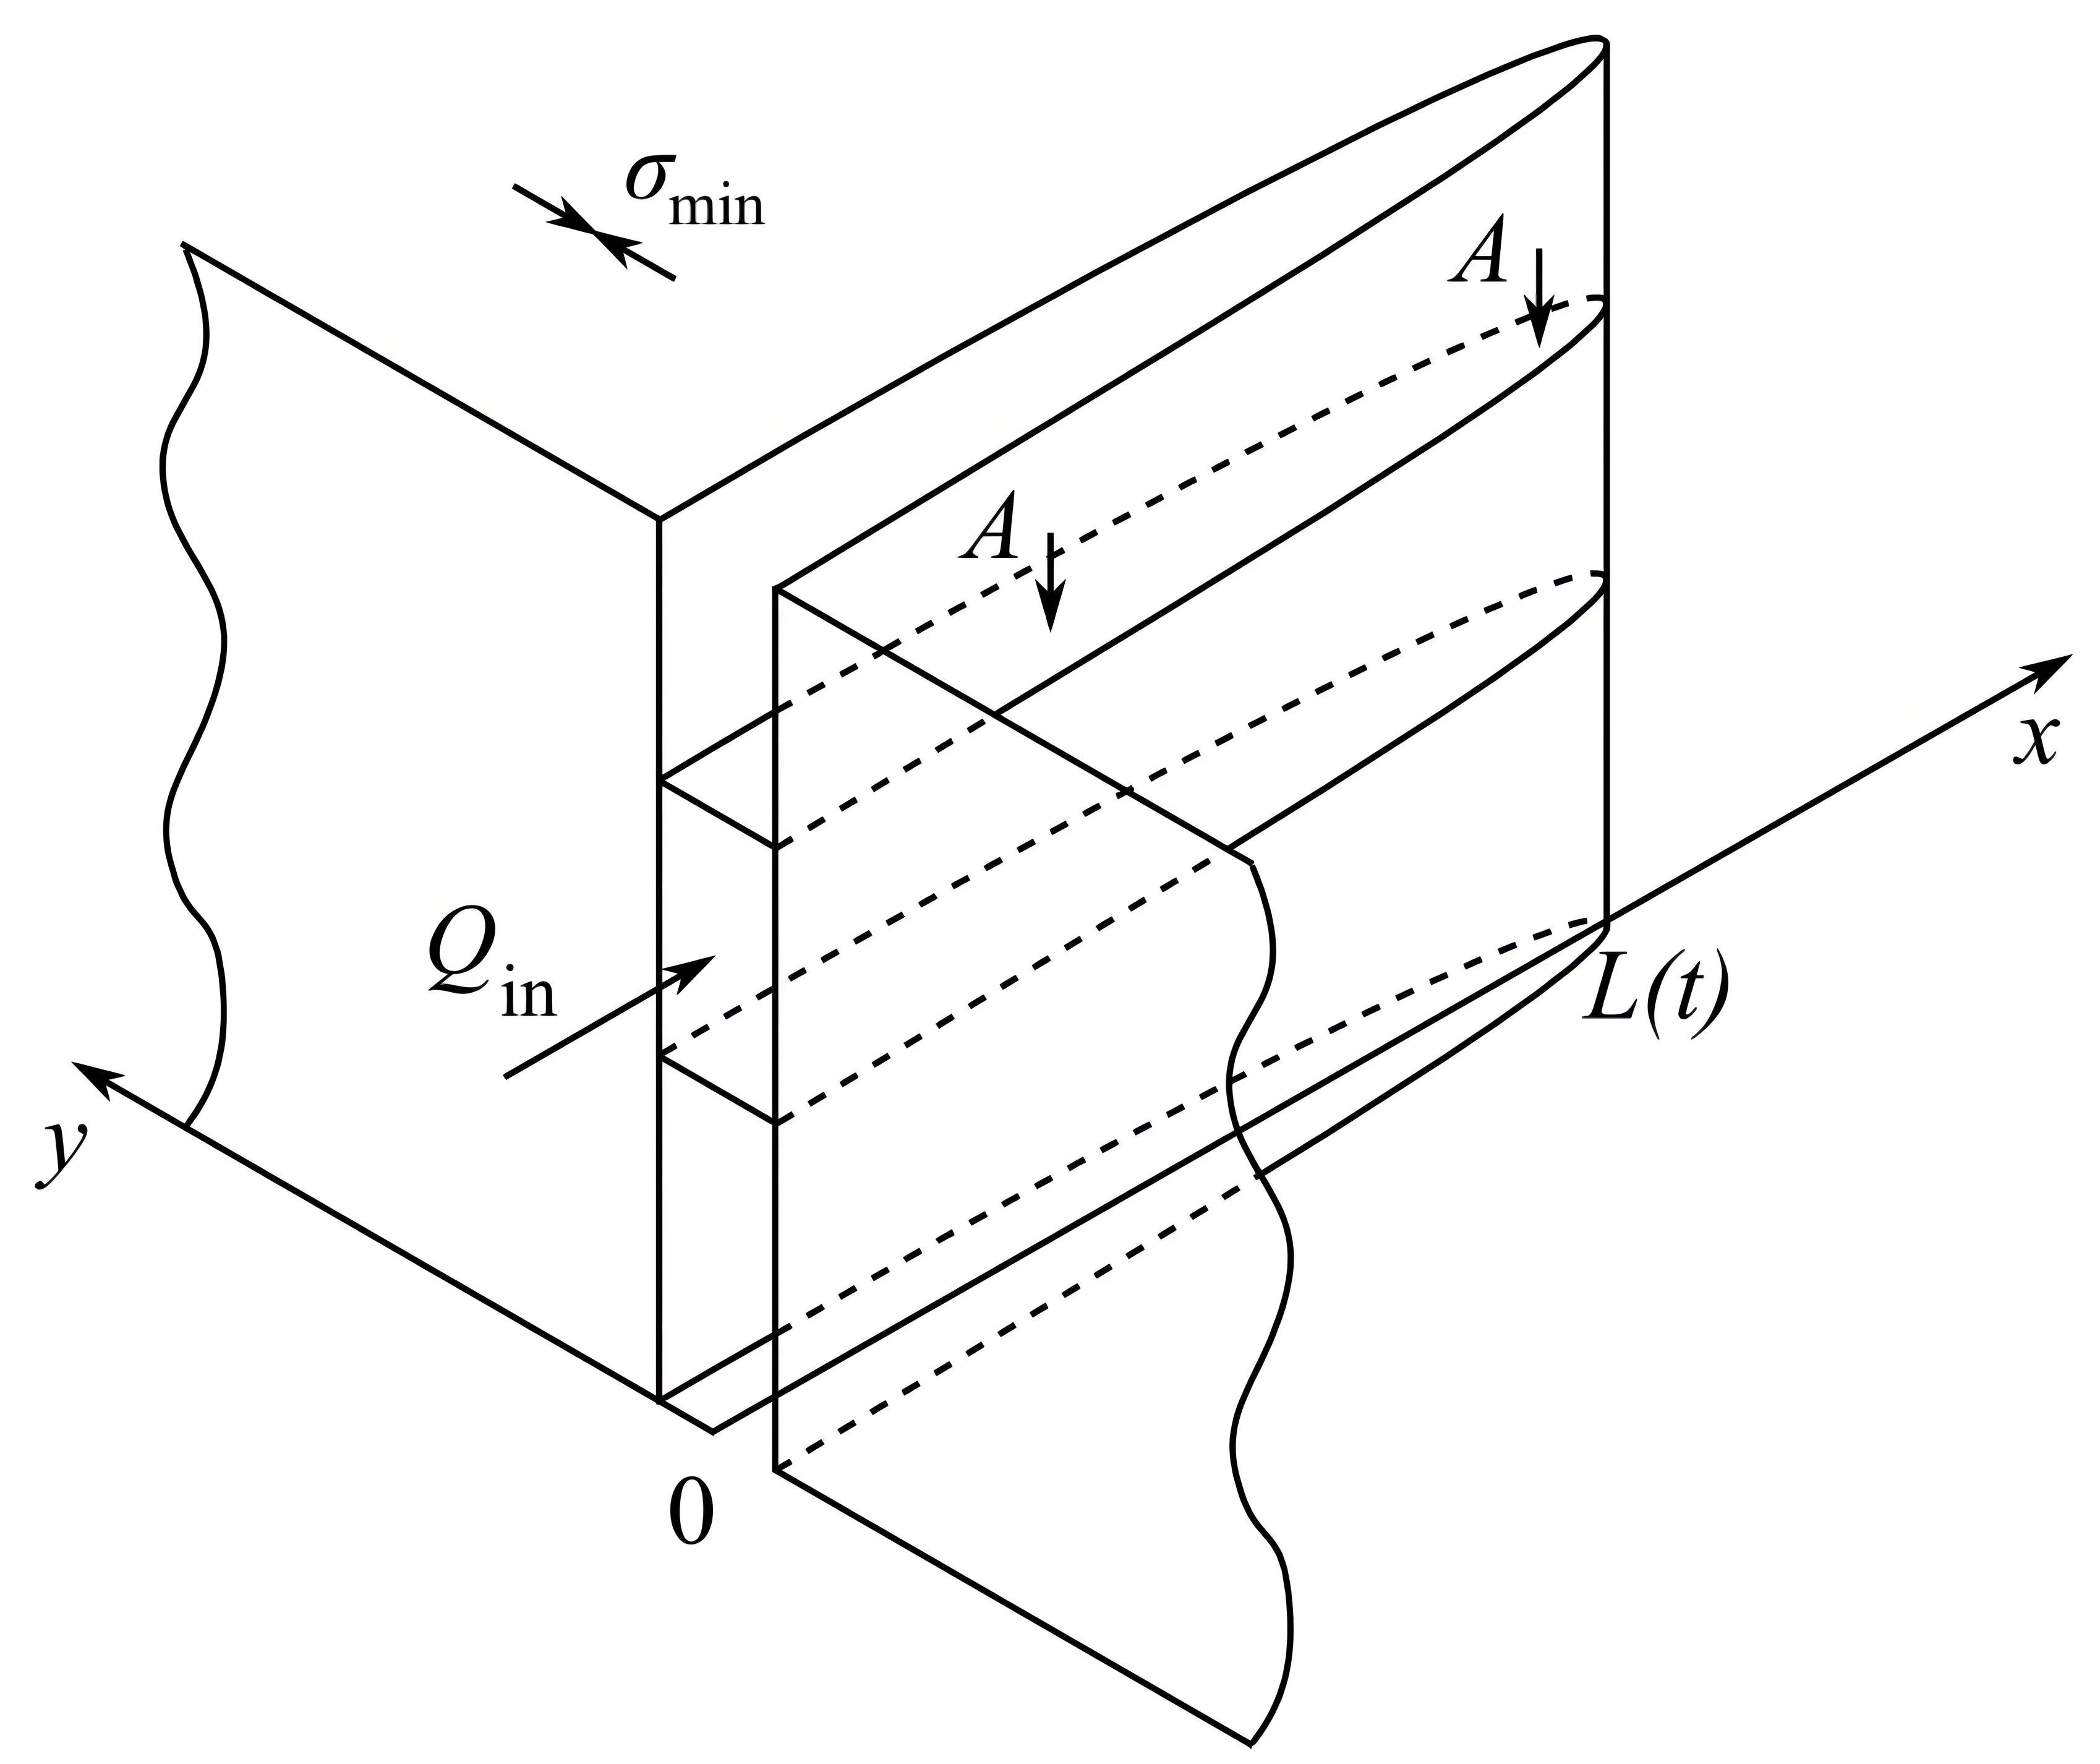
\includegraphics[width=6cm]{kgd_model_3D.jpg}
\end{textblock*}

\begin{textblock*}{8cm}(6.5cm,6.1cm)
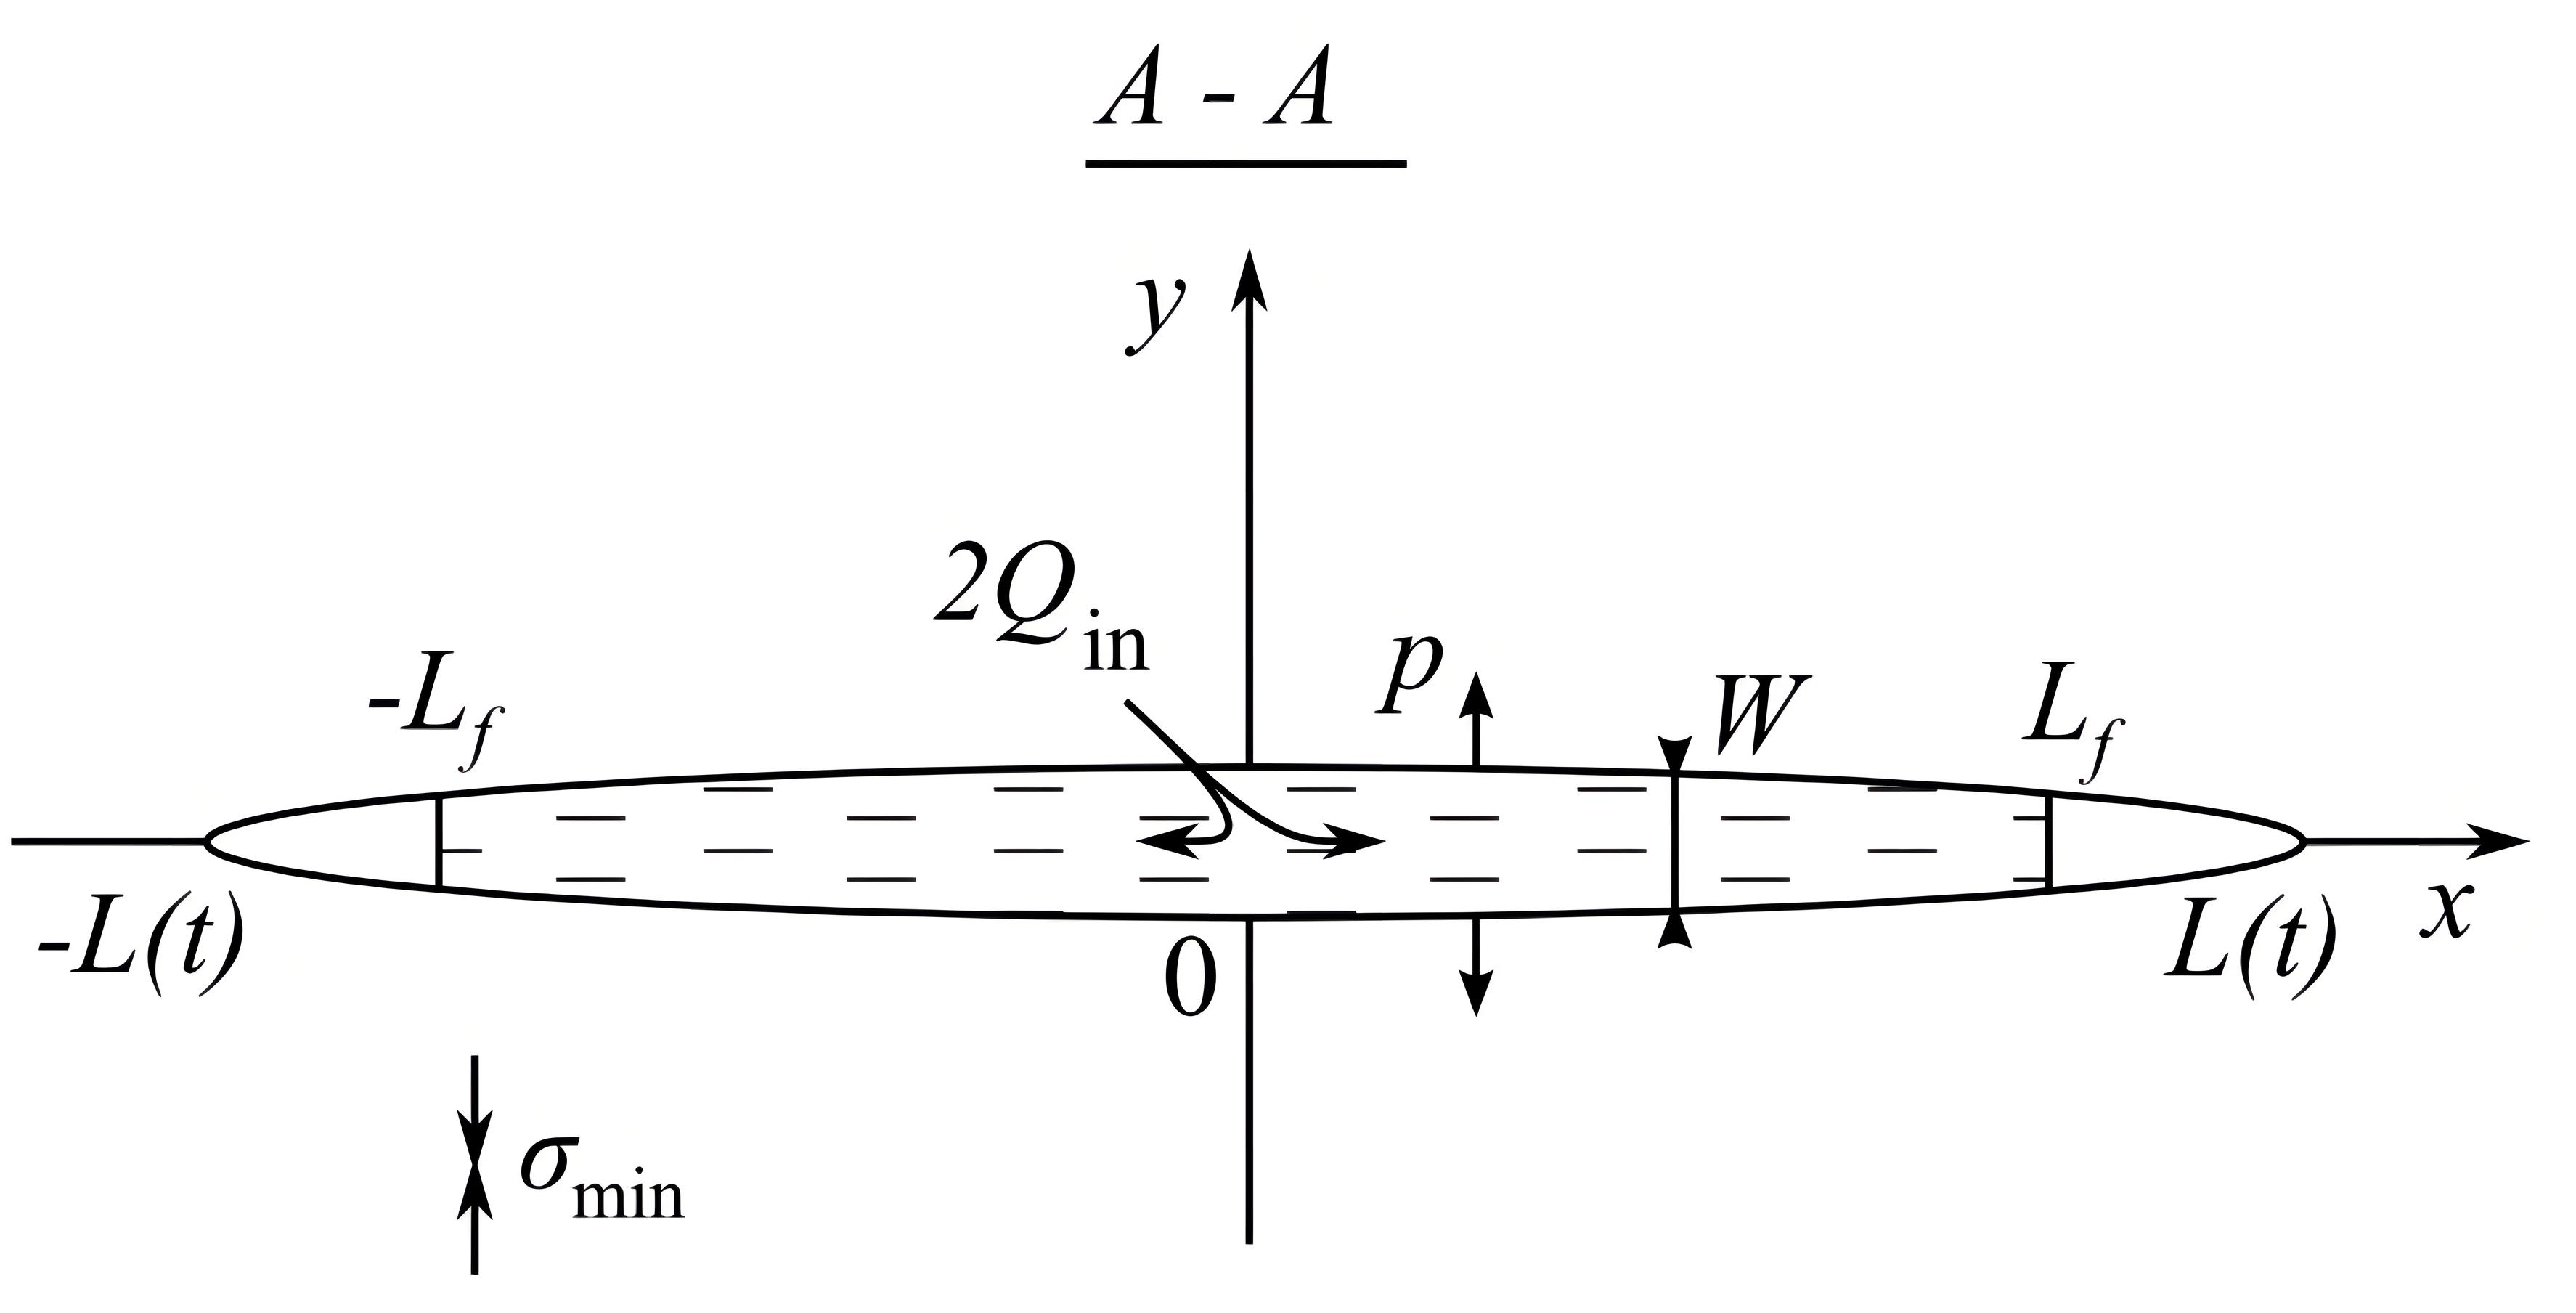
\includegraphics[width=6cm]{kgd_model_A-A_plane.jpg}
\end{textblock*}

\begin{textblock*}{6cm}(0.5cm,8.7cm)
\tiny
\textcolor{lit_gray}{E.V. Dontsov. An approximate solution for a plane strain hydraulic fracture that accounts for fracture toughness, fluid viscosity, and leak-off. \emph{Int. J. Fract.}, 205:221-237, 2017}
\end{textblock*}

\normalsize

\end{frame}

\begin{frame}
\frametitle{Модель радиальной трещины}

\scriptsize

\begin{textblock*}{7cm}(0.5cm,0.8cm)
$$
\begin{cases}
\dfrac{\partial w}{\partial t}+\dfrac{1}{r}\dfrac{\partial}{\partial r}\!\left(rq\right)+\dfrac{C'}{\sqrt{t-t_0(r)}}=Q_0\delta(r),\\[15pt]
q=-\dfrac{w^3}{\mu'}\dfrac{\partial p_n}{\partial r},\\[5pt]
p_n(r,t)=-\dfrac{E'}{2\pi R}\displaystyle\int\limits_{0}^{R(t)}M\!\left(\dfrac{r}{R},\dfrac{r'}{R}\right)\dfrac{\partial w(r',t)}{\partial r'}dr',\\[20pt]
\displaystyle\lim_{r\to R}\dfrac{w}{(R-r)^{1/2}}=\dfrac{K'}{E'},
\end{cases}
$$
где $C'=2C_l$; $\,\,\,\mu'=12\mu$; $\,\,\,E'=\dfrac{E}{1-\nu^2}$; $\,\,\,K'=\dfrac{8K_{Ic}}{\sqrt{2\pi}}$;
$$
M(\rho,s)=
\begin{cases}
\dfrac{1}{\rho}\,K\!\left(\dfrac{s^2}{\rho^2}\right)+\dfrac{\rho}{s^2-\rho^2}\,E\!\left(\dfrac{s^2}{\rho^2}\right)\\\ \\
\dfrac{s}{s^2-\rho^2}\,E\!\left(\dfrac{\rho^2}{s^2}\right)
\end{cases}
$$
\end{textblock*}

\begin{textblock*}{7cm}(7cm,1cm)
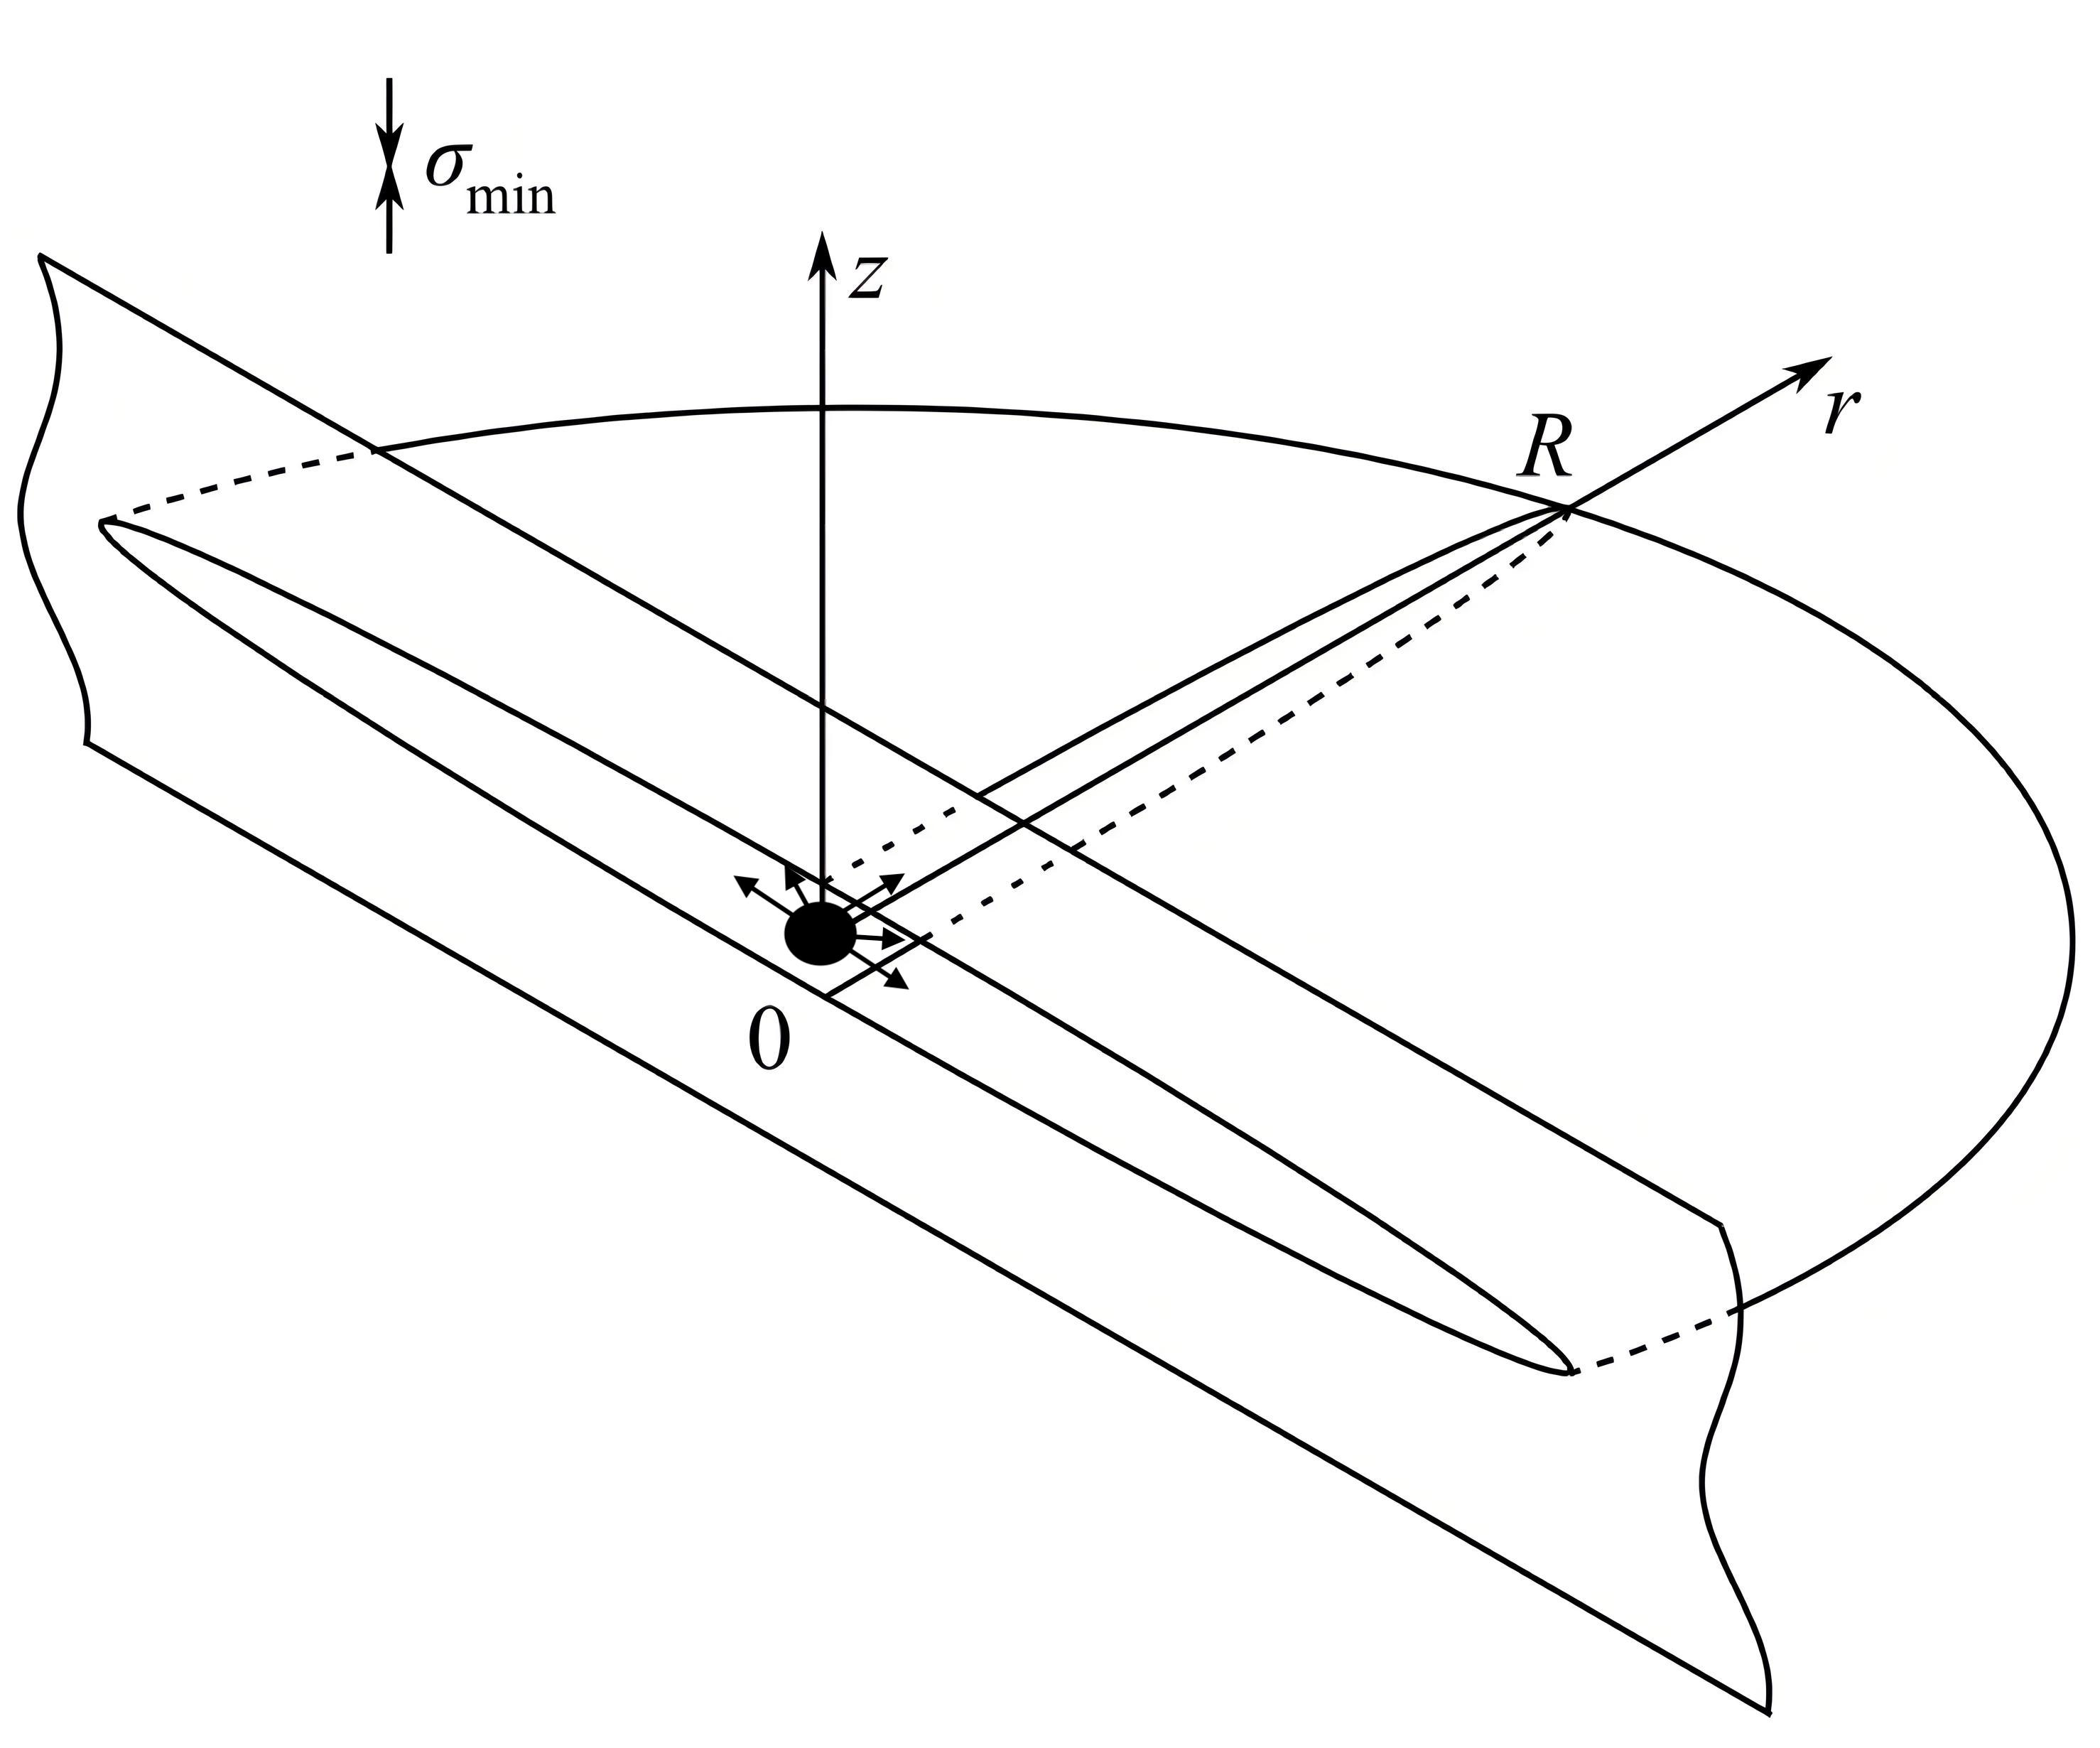
\includegraphics[width=5.5cm]{radial_model_3D.jpg}
\end{textblock*}

\begin{textblock*}{7cm}(7.4cm,5.7cm)
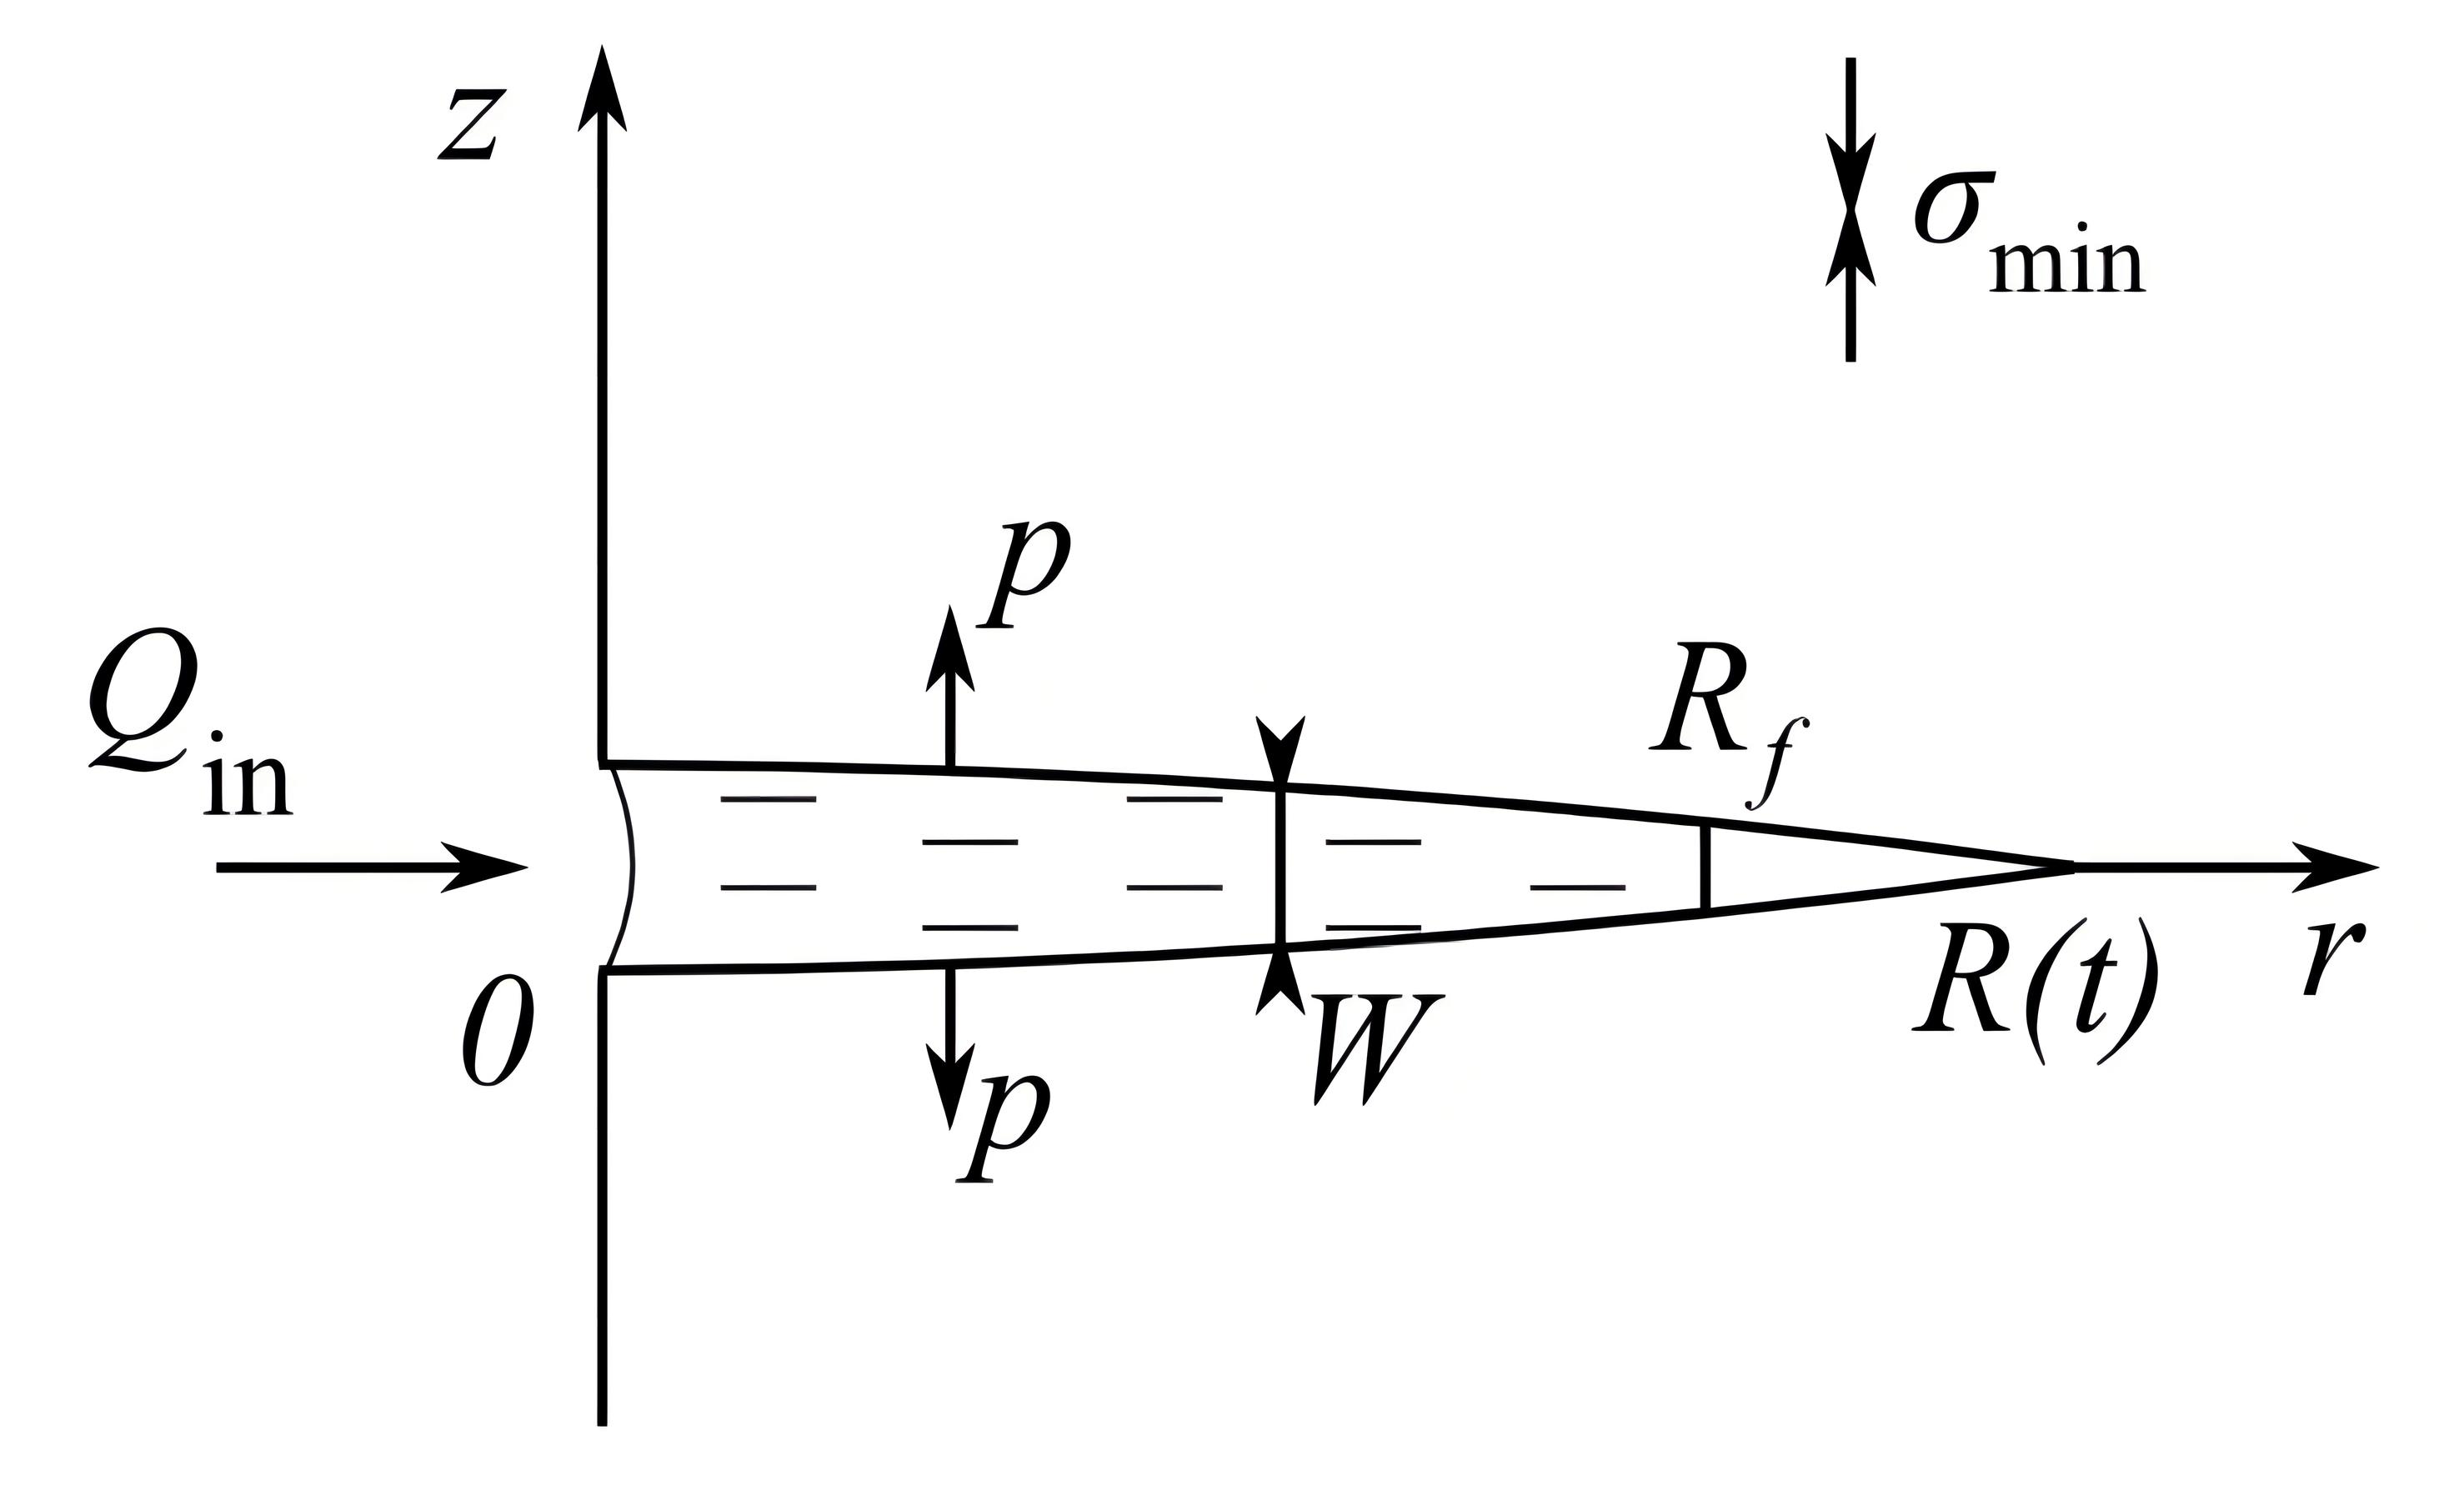
\includegraphics[width=5.2cm]{radial_model_A-A_plane.jpg}
\end{textblock*}

\begin{textblock*}{6cm}(0.5cm,8.7cm)
\tiny
\textcolor{lit_gray}{E.V. Dontsov. An approximate solution for a penny-shaped hydraulic fracture that accounts for fracture toughness, fluid viscosity, and leak-off. \emph{R. Soc. Open Sci.}, 3:160737, 2016}
\end{textblock*}

\normalsize

\end{frame}


\begin{frame}
\frametitle{Модель Перкинса-Керна-Нордгрена (модель PKN)}

\scriptsize

\begin{textblock*}{7cm}(0.5cm,1cm)
$$
\begin{cases}
\dfrac{\partial\bar{w}}{\partial t}+\dfrac{\partial\bar{q}_x}{\partial x}+\dfrac{C'}{\sqrt{t-t_0(x)}}=\dfrac{Q_0}{H}\delta(x),\\[15pt]
\bar{q}_x=-\dfrac{\bar{w}^3}{\pi^2\mu}\dfrac{\partial p_n}{\partial x},\\[15pt]
p_n(x,t)=\dfrac{2E'}{\pi^2H}\displaystyle\int\limits_{-L(t)}^{L(t)}\bar{w}(x',t)\dfrac{dG(2(x'-x)/H)}{dx'}dx',\\[22pt]
\displaystyle\lim_{x\to L}\dfrac{w}{(L-x)^{1/2}}=\dfrac{K'}{E'},
\end{cases}
$$
где $C'=2C_l$; $\,\,\,\mu'=12\mu$; $\,\,\,E'=\dfrac{E}{1-\nu^2}$; $\,\,\,K'=\dfrac{8K_{Ic}}{\sqrt{2\pi}}$;
\end{textblock*}

\begin{textblock*}{7cm}(2.1cm,7.2cm)
$$
G(s)=\frac{\sqrt{1+s^2}}{s}\,E\!\left(\frac{1}{1+s^2}\right)
$$
\end{textblock*}

\begin{textblock*}{7cm}(7.4cm,1.5cm)
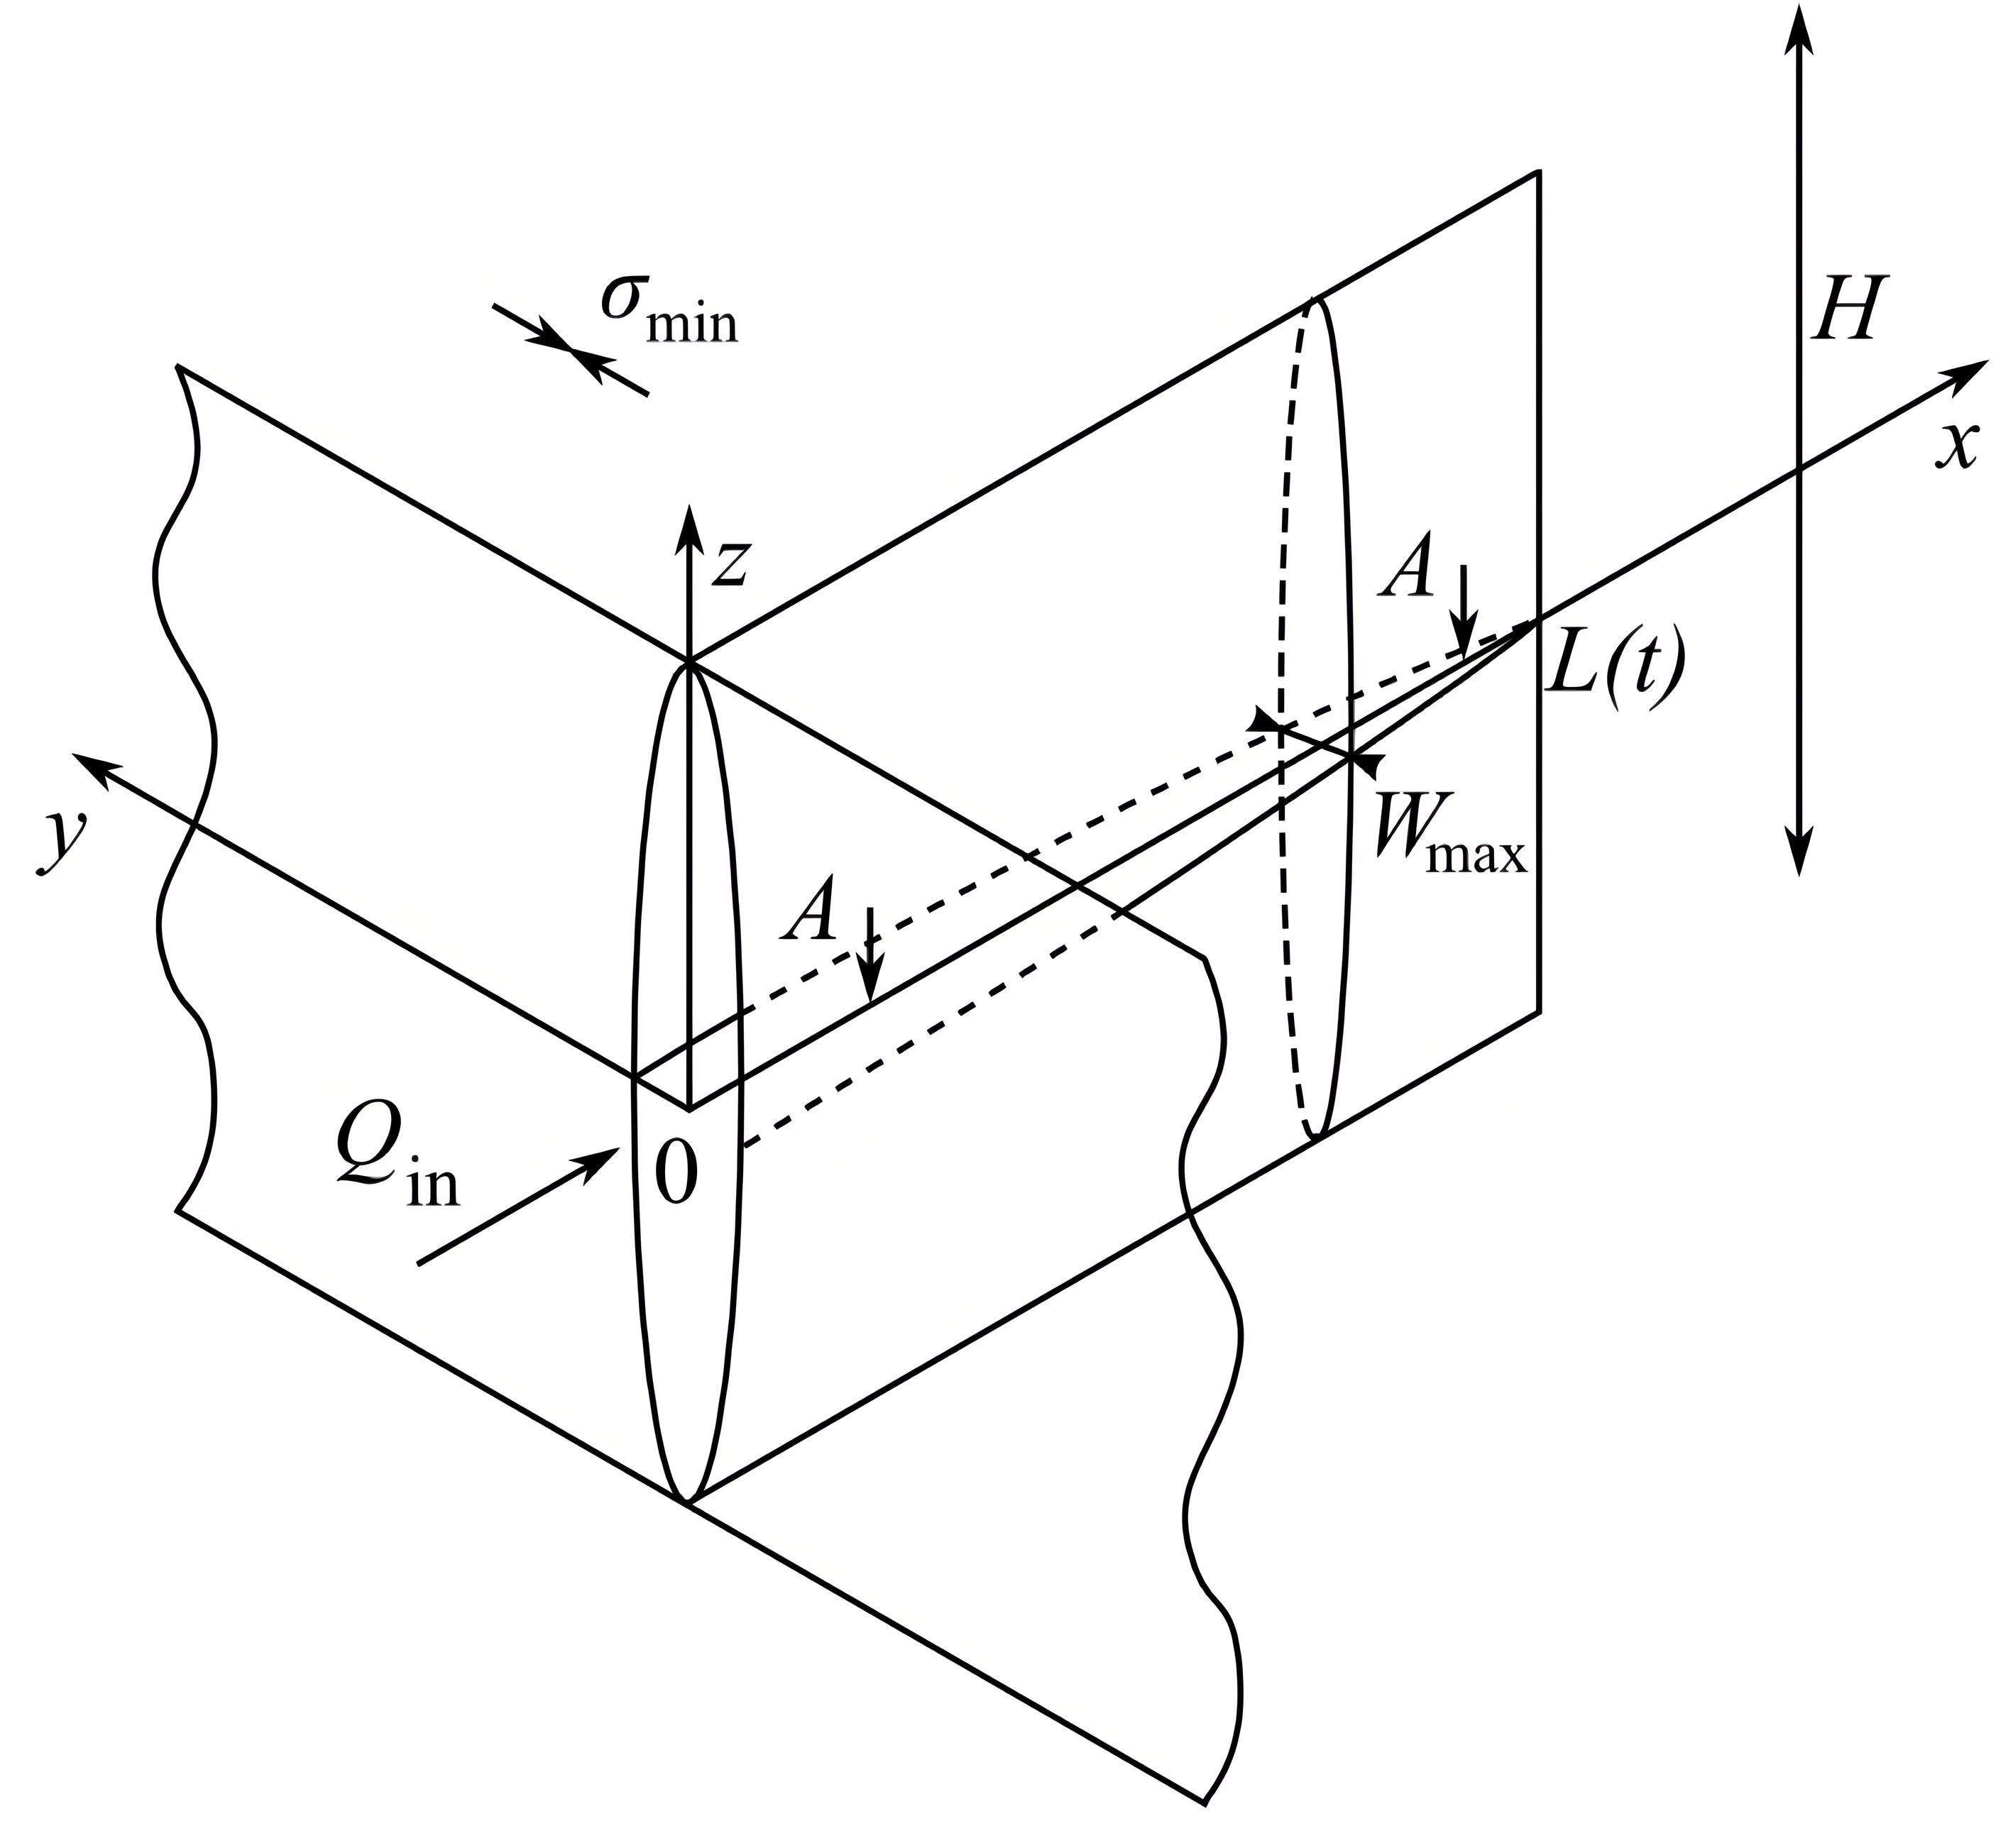
\includegraphics[width=5.2cm]{pkn_model_3D.jpg}
\end{textblock*}

\begin{textblock*}{7cm}(7.5cm,6.3cm)
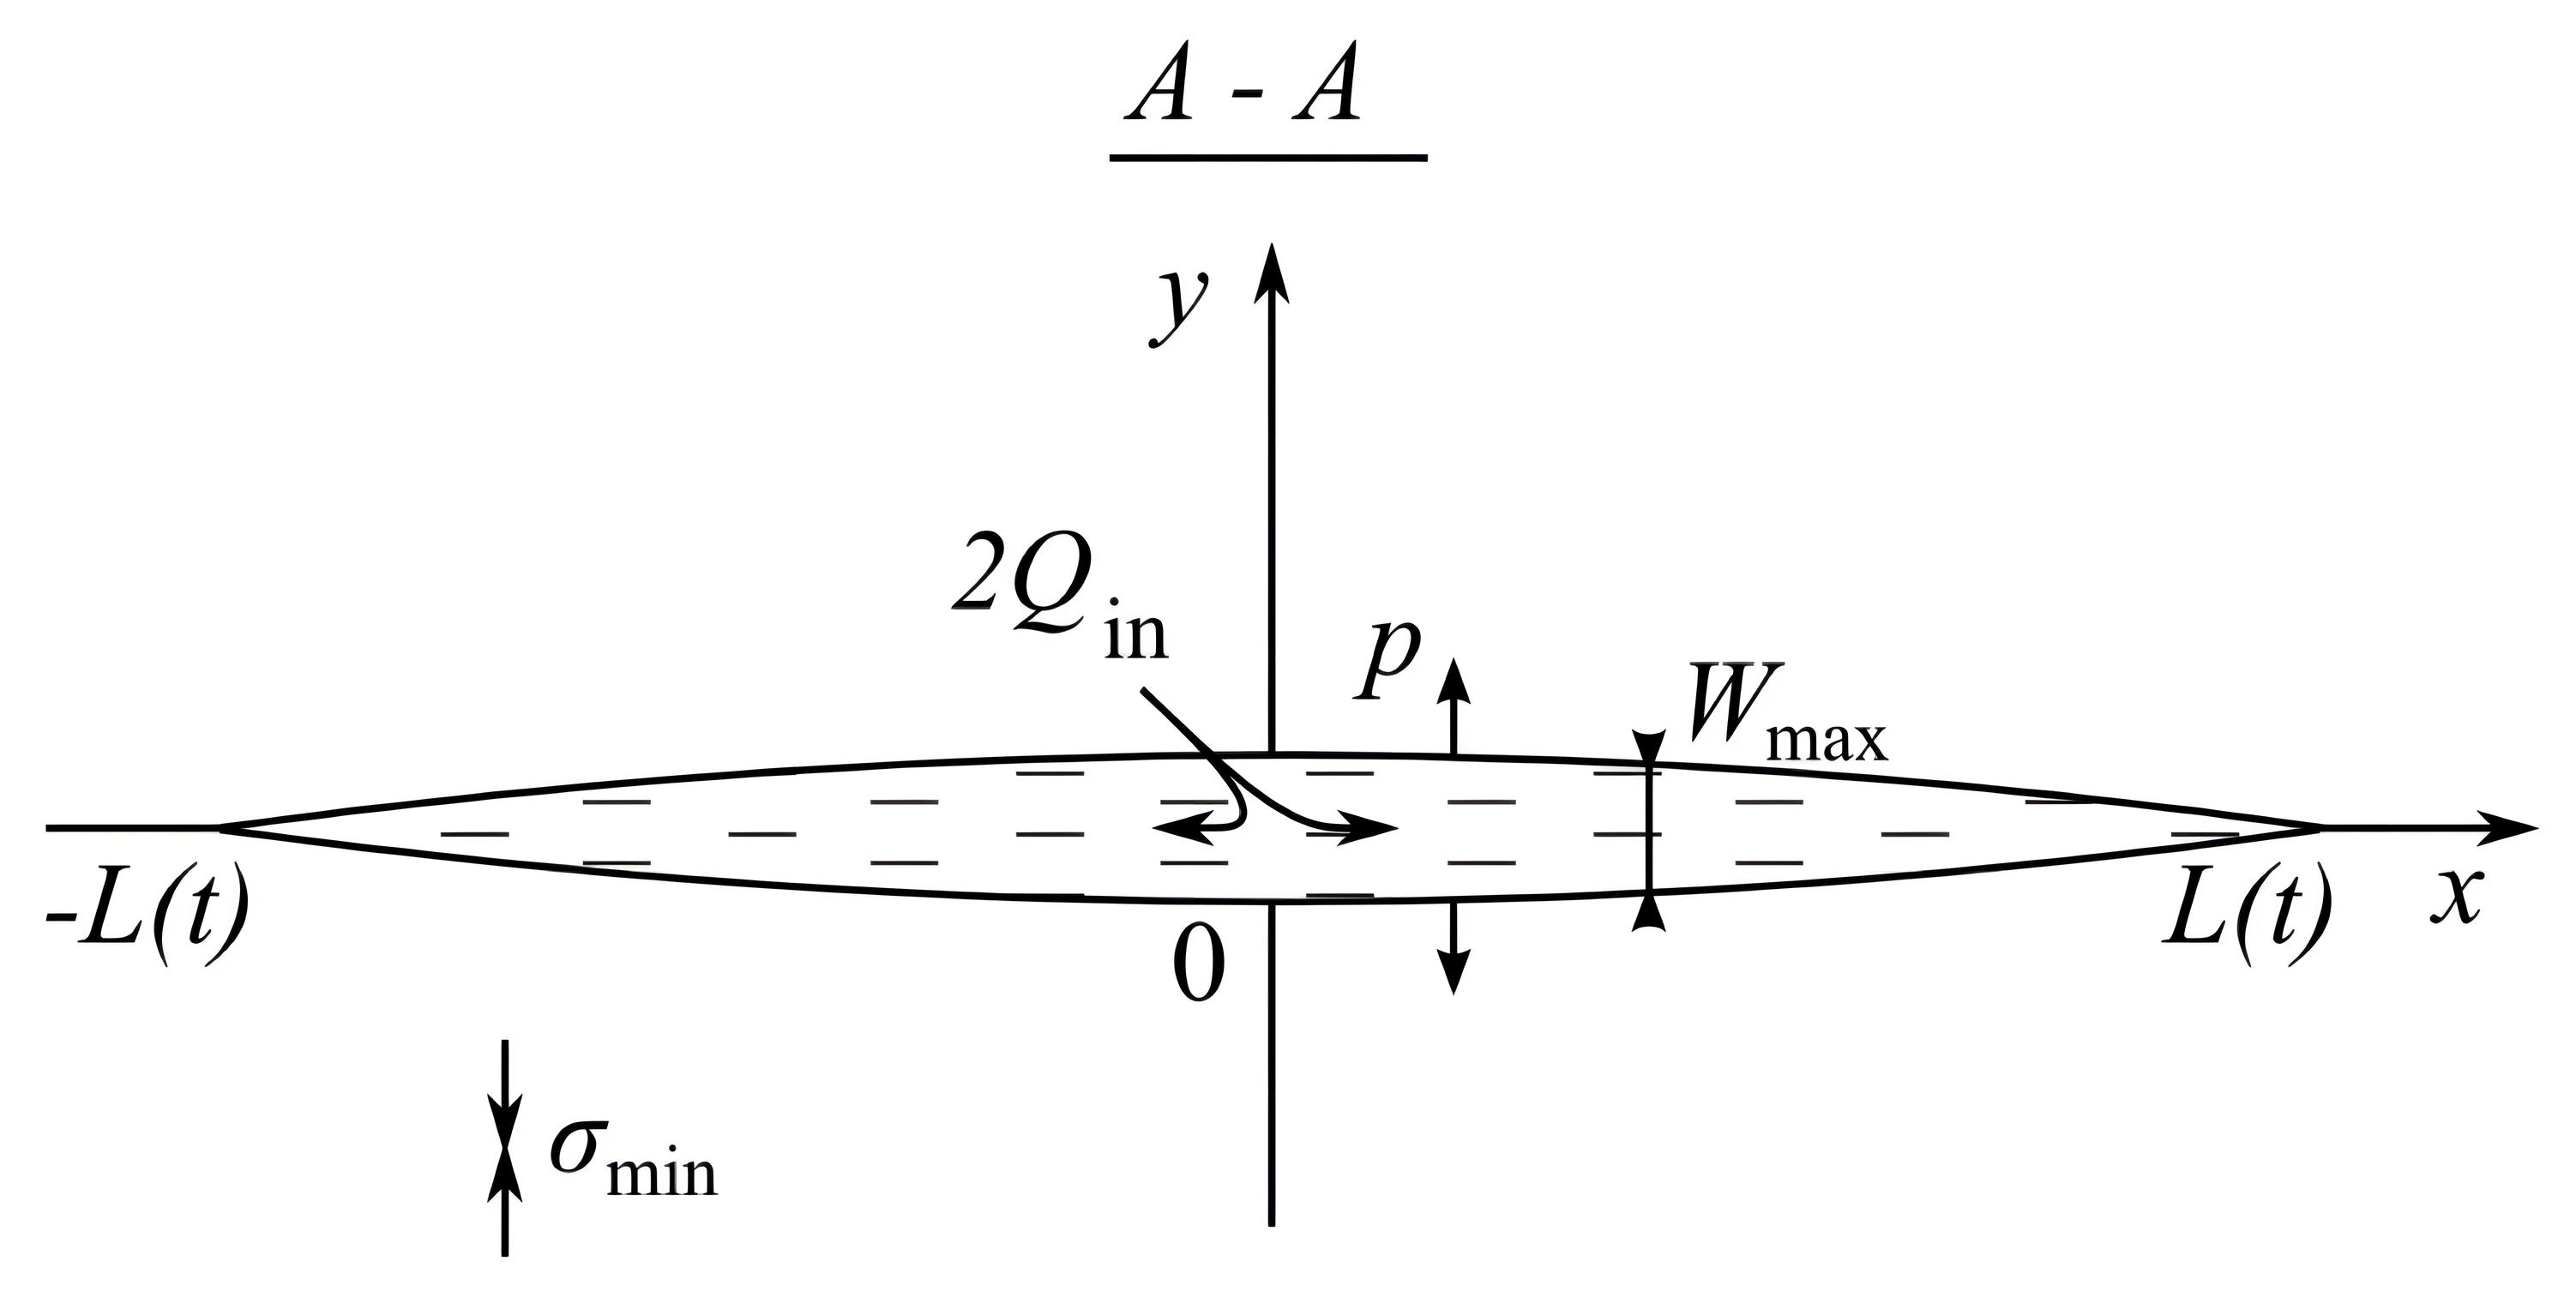
\includegraphics[width=5cm]{pkn_model_A-A_plane.jpg}
\end{textblock*}

\begin{textblock*}{3.7cm}(0cm,6.8cm)
\tiny
$$
\boxed{
\bar{w}(x)=\frac{1}{H}\!\int\limits_{-H/2}^{H/2}{w(x,z)dz}
}
$$
\end{textblock*}

\begin{textblock*}{7cm}(6cm,1.2cm)
\tiny
$$
w(x,z)=\frac{4}{\pi}\bar{w}(x)\sqrt{1-\left(\frac{2z}{H}\right)^2}
$$
\end{textblock*}

\begin{textblock*}{6cm}(0.5cm,8.9cm)
\tiny
\textcolor{lit_gray}{E.V. Dontsov. Analysis of a constant height hydraulic fracture, arXiv:2110.13088v1 [physics.geo-ph], 25 Oct 2021}
\end{textblock*}

\normalsize

\end{frame}


\begin{frame}
\frametitle{Параметрическая карта решения модели PKN}

\begin{textblock*}{7cm}(5.5cm,1.2cm)
\tiny
$$
\Omega=\frac{\bar{w}}{w_{*}}\,\,\,\,\,;\,\,\,\,\,\lambda=\frac{l}{l_{*}}\,\,\,\,\,;\,\,\,\,\,\tau=\frac{t}{t_{*}}\,\,\,\,\,;\,\,\,\,\,\xi=\frac{x}{l(t)}
$$
\normalsize
\end{textblock*}

\begin{textblock*}{7cm}(5.5cm,2.2cm)
\tiny
$$
w_{*}=\frac{\left(\pi H\right)^{1/2}K_{Ic}}{E'}\,\,\,\,\,;\,\,\,\,\,l_{*}=\frac{H^2K_{Ic}^4}{2\pi E'^3\mu Q_0}
$$
\normalsize
\end{textblock*}

\begin{textblock*}{7cm}(5.5cm,3.2cm)
\tiny
$$
t_{*}=\frac{H^{7/2}K_{Ic}^5}{2\pi^{1/2}E'^4\mu Q_0^2}\,\,\,\,\,;\,\,\,\,\,\phi=\left(\frac{H^5K_{Ic}^6C'^4}{4\pi^3E'^4\mu^2Q_0^4}\right)^{1/4}
$$
\normalsize
\end{textblock*}

\begin{textblock*}{6cm}(6cm,4.5cm)
\scriptsize
\textcolor{red}{
$K$-режим = доминирование трещиностойкости и отсутствие утечек (пренебрегаем вязкостью)
}
\normalsize
\end{textblock*}

\begin{textblock*}{6cm}(6cm,5.6cm)
\scriptsize
\textcolor{magenta}{
$\tilde{K}$-режим = доминирование трещиностойкости и большие утечки (пренебрегаем вязкостью)
}
\normalsize
\end{textblock*}

\begin{textblock*}{6.5cm}(6cm,6.8cm)
\scriptsize
\textcolor{blue}{
$M$-режим = доминирование вязкости и отсутствие утечек (пренебрегаем трещиностойкостью)
}
\normalsize
\end{textblock*}

\begin{textblock*}{6cm}(6cm,7.8cm)
\scriptsize
\textcolor{new_green}{
$\tilde{M}$-режим = доминирование вязкости и большие утечки (пренебрегаем трещиностойкостью)
}
\normalsize
\end{textblock*}

\begin{textblock*}{4.5cm}(0.5cm,5.2cm)
\scriptsize
\renewcommand{\baselinestretch}{0.7}
В данной работе предполагается, что трещины автоГРП распространяются в режиме больших утечек и доминирования трещиностойкости (пренебрегаем вязкостью).
В этом режиме решение для среднего раскрытия:
\vspace*{-3mm}
$$
\bar{w}_{\tilde{K}}=\frac{K_{Ic}\sqrt{\pi H}}{E'}
$$
\normalsize
\end{textblock*}



\begin{textblock*}{5cm}(0.5cm,1.5cm)
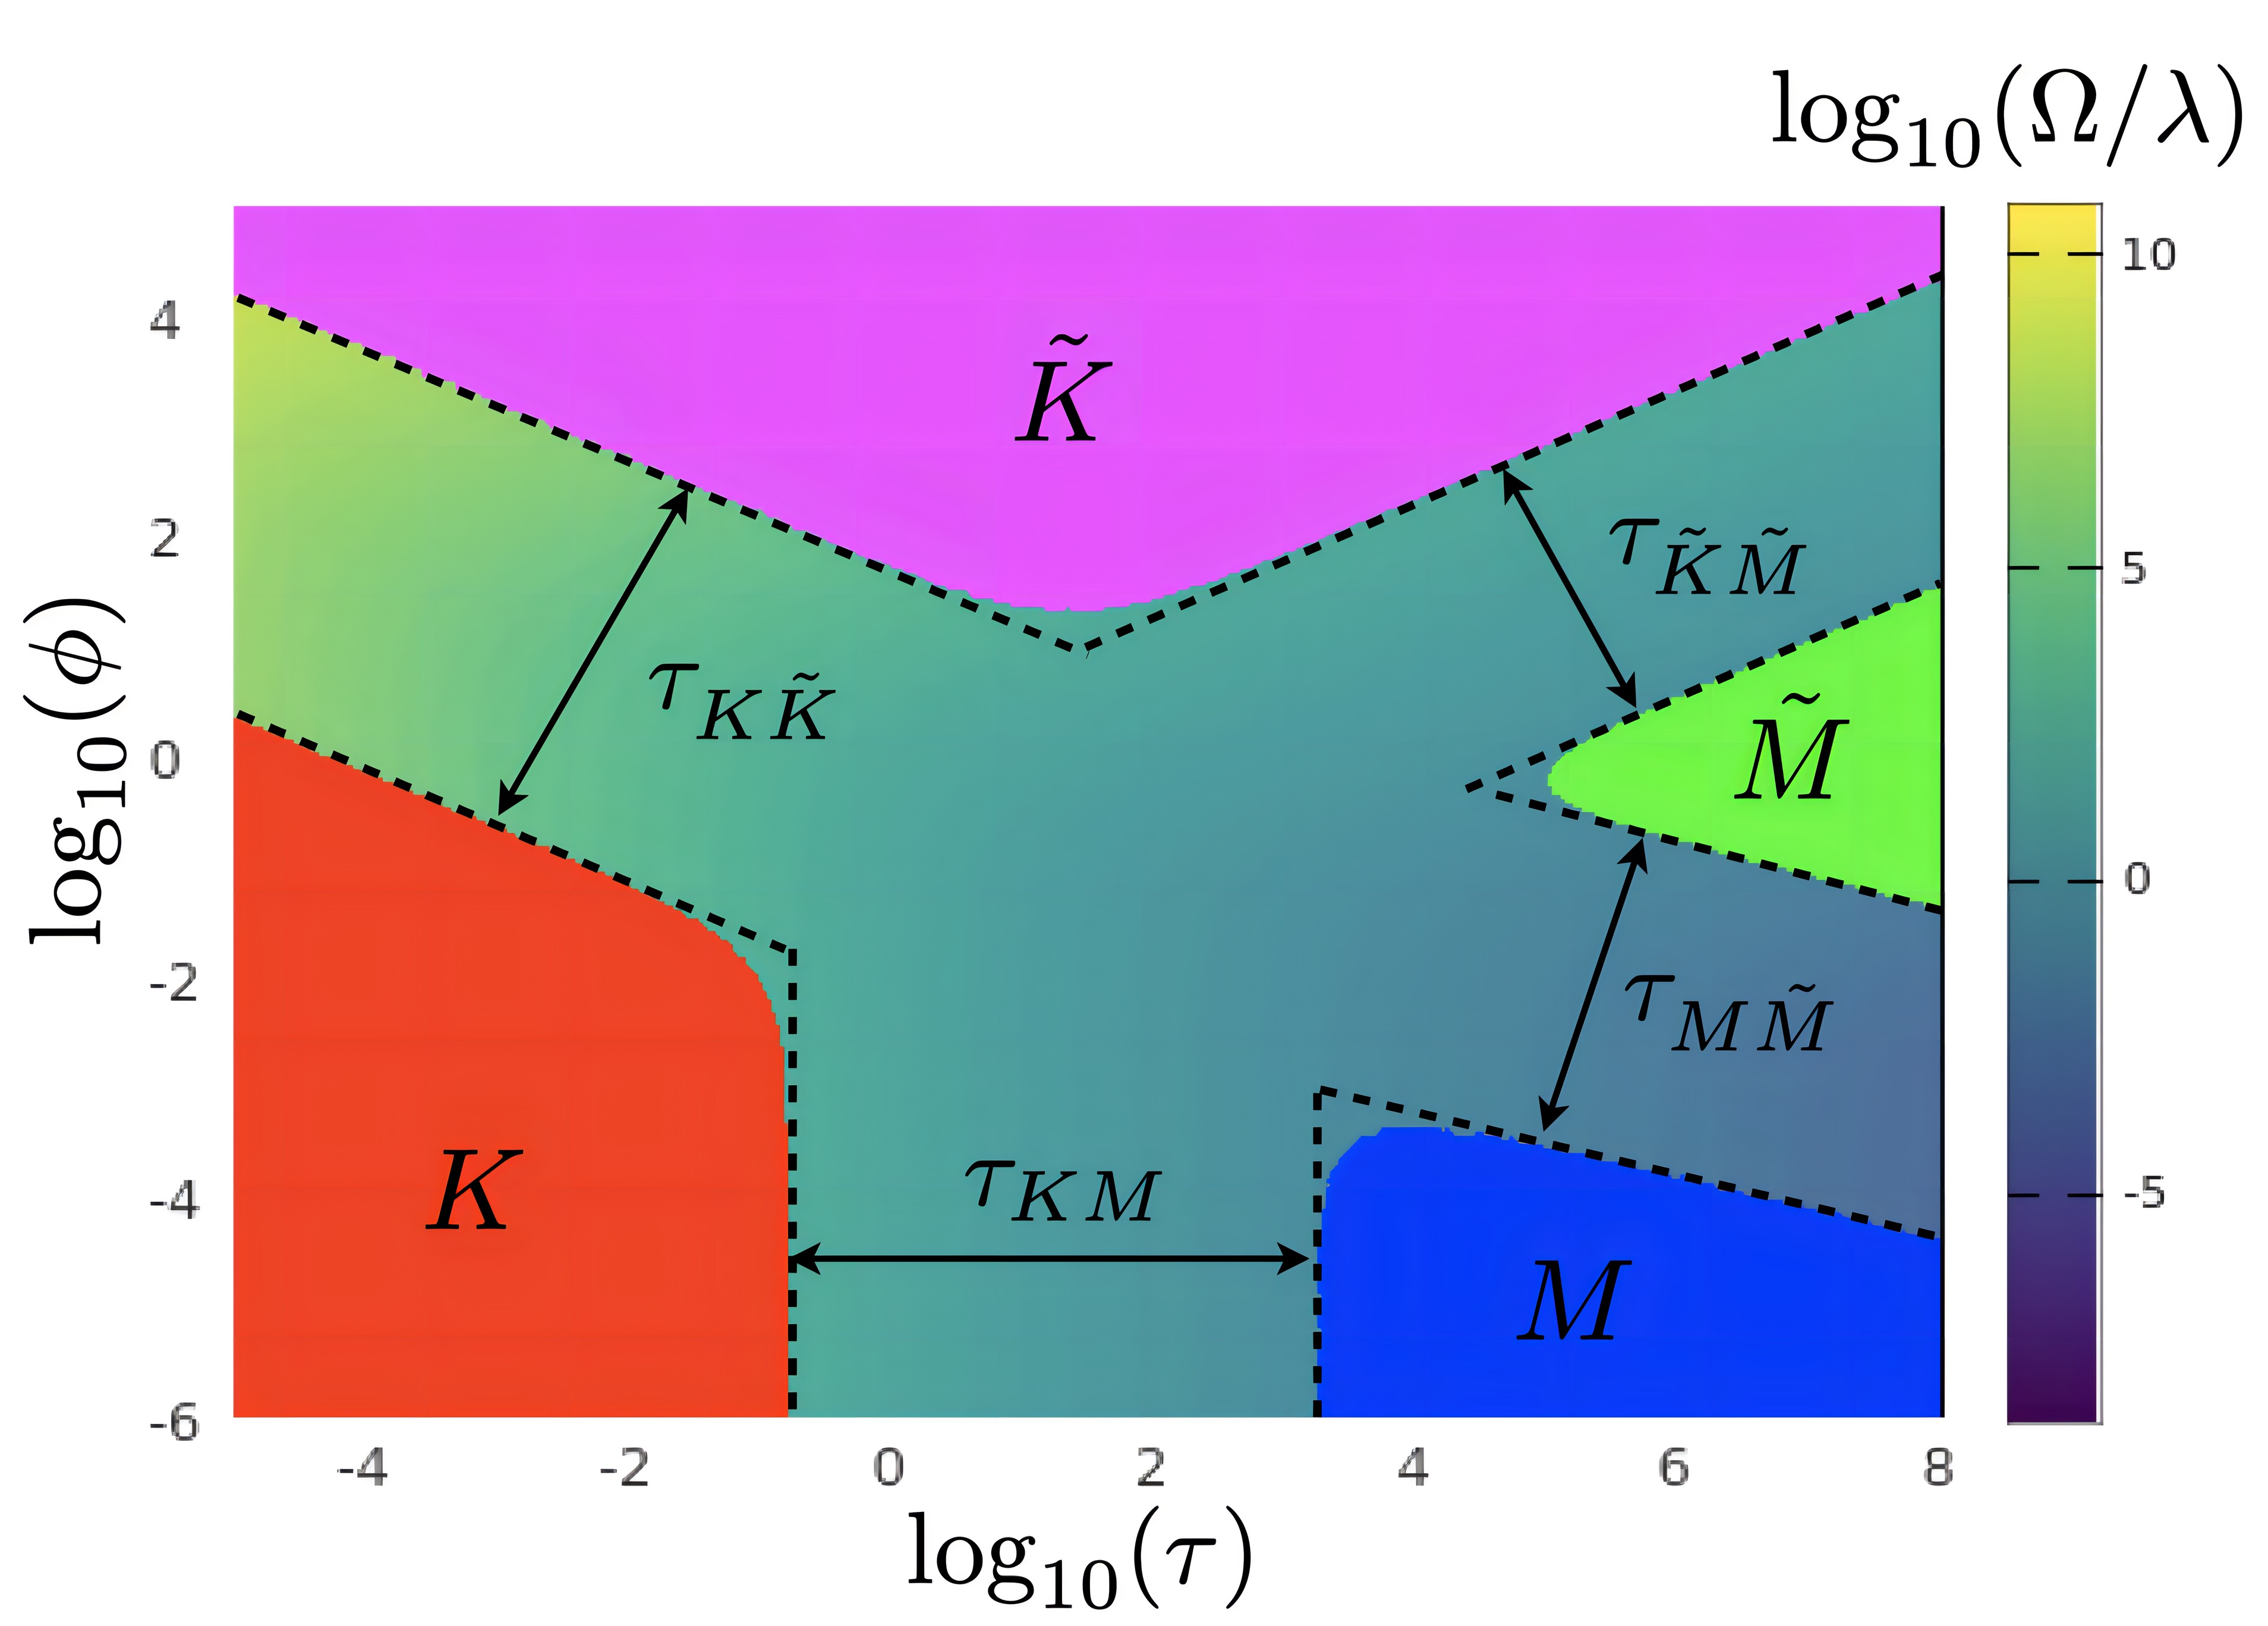
\includegraphics[width=5cm]{pkn_parametric_space.jpg}
\end{textblock*}

\begin{textblock*}{6cm}(0.5cm,8.9cm)
\tiny
\textcolor{lit_gray}{E.V. Dontsov. Analysis of a constant height hydraulic fracture, arXiv:2110.13088v1 [physics.geo-ph], 25 Oct 2021}
\end{textblock*}

\end{frame}



\begin{frame}
\frametitle{Схема перераспределения потоков между трещинами гидроразрыва и законы Кирхгофа}

\begin{textblock*}{11cm}(1cm,1.5cm)
%\tiny Подпись к рисунку
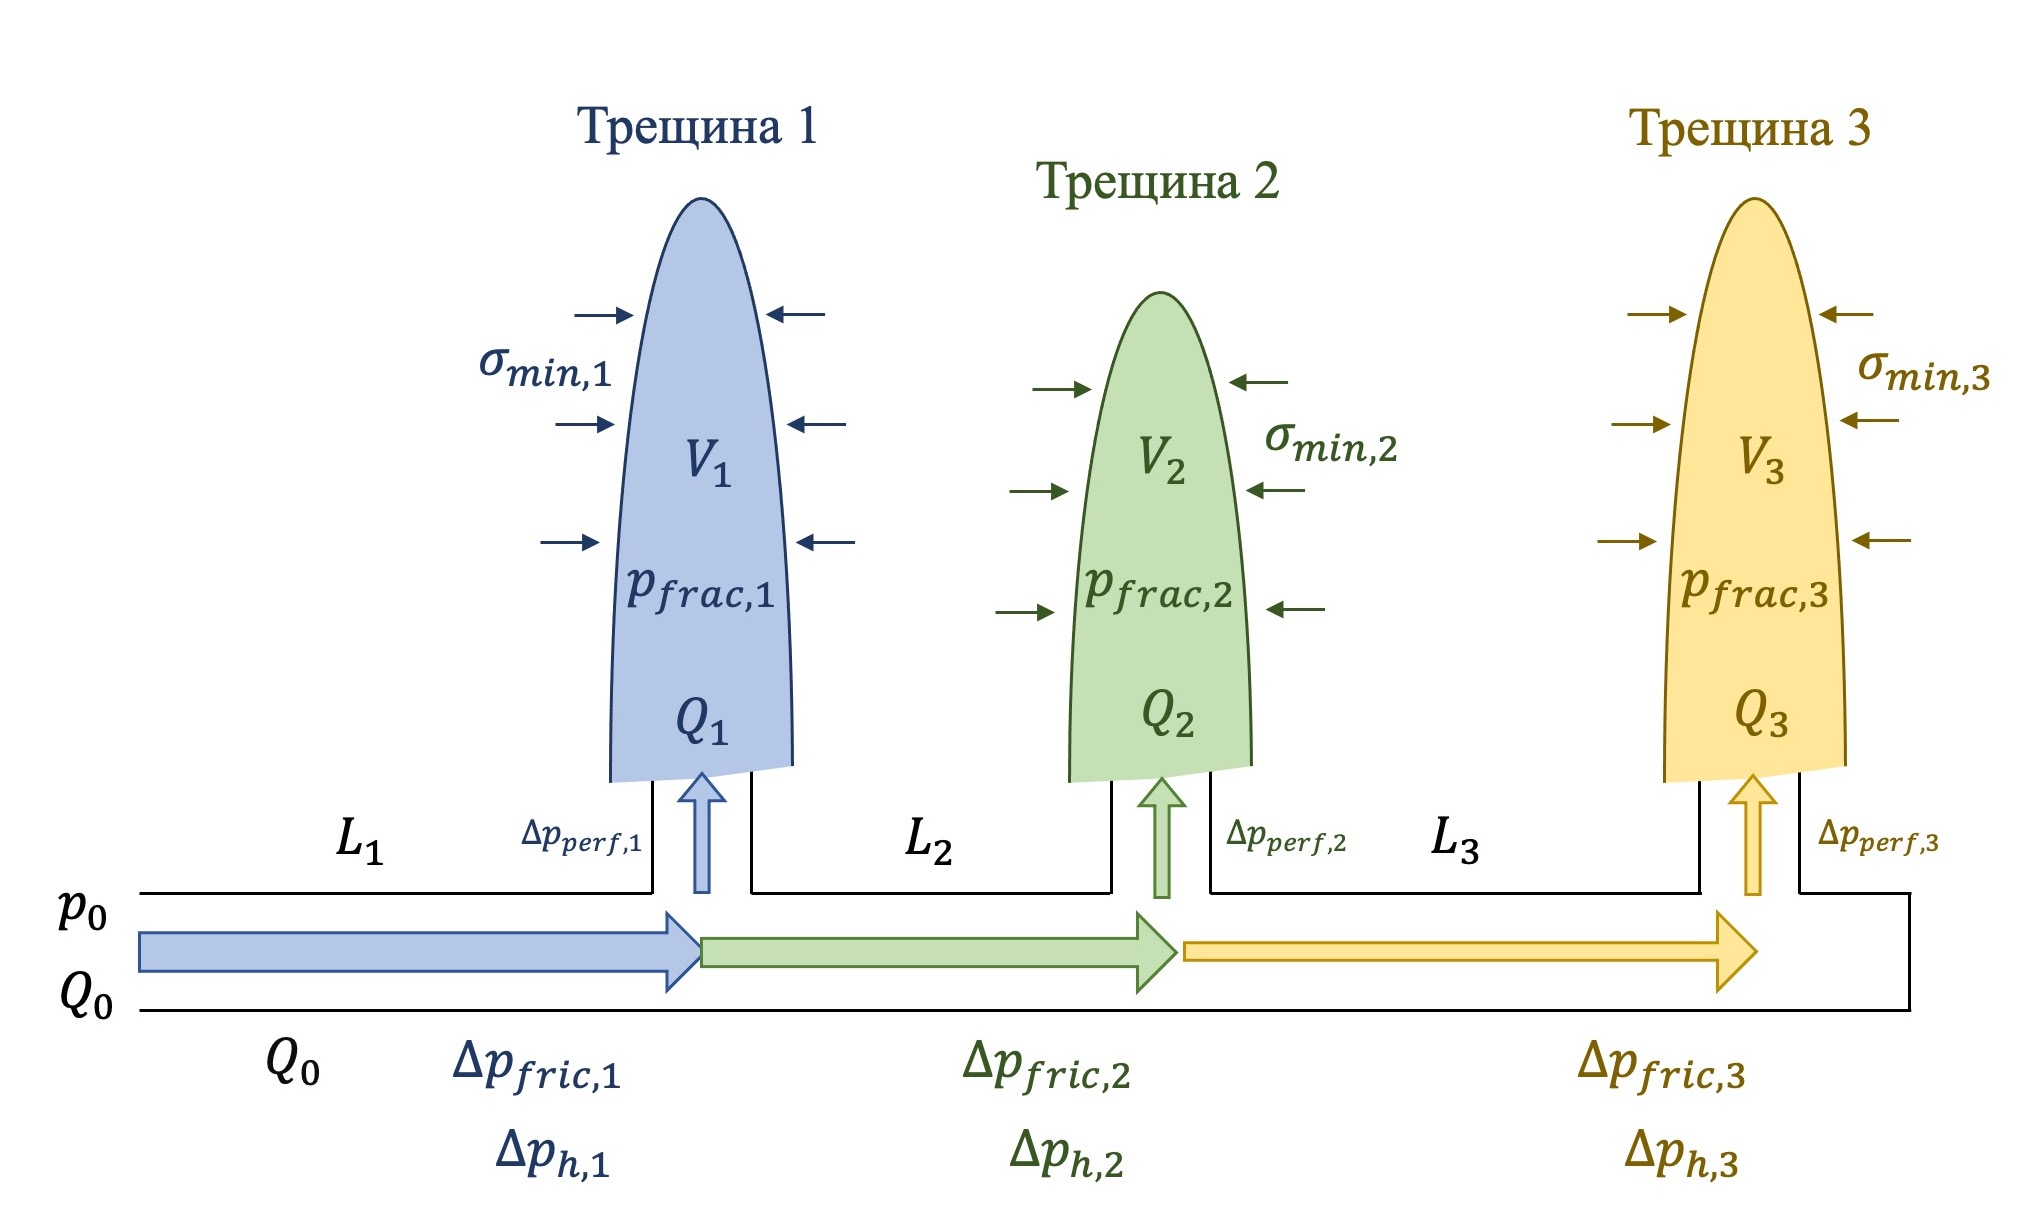
\includegraphics[width=10cm]{flow_distribution_scheme.jpg}
\end{textblock*}

\begin{textblock*}{4cm}(-0.5cm,7.5cm)
$$\boxed{Q_0=\sum\limits_{i=1}^{N}Q_i}$$
\end{textblock*}

\begin{textblock*}{11cm}(2.2cm,7.5cm)
$$\boxed{p_0=\sigma_{\text{min},i}+p_{\text{net},i}+\Delta p_{\text{perf},i}-\sum_{j=1}^{i}{\Delta p_{h,\,j}}+\sum_{j=1}^{i}\Delta p_{\text{fric},\,j}}$$
\end{textblock*}

\end{frame}


\begin{frame}
\frametitle{Чистое давление в трещинах PKN}
$$
p_{\text{net},i}(Q_i)=a_iQ_i^{\frac{n}{2n+3}}V_i^{\frac{1}{2n+3}},
$$\\
\small
где $a_i=\left(\dfrac{(n+3)(2n+1)^n \cdot K\cdot (E_i')^{2n+2}}{\pi\, 2^{2n}n^n\phi^n h_i^{3n+3}}\right)^{\!\frac{1}{2n+3}}$ -- параметр жёсткости,\newline\\
$Q_i$ и $V_i$ -- расход на $i$-ой трещине и объём $i$-ой трещины;\newline
$K$ и $n$ -- реологические параметры степенной жидкости;\newline
$E_i'$ -- модуль плоской деформации породы вблизи $i$-ой трещины;\newline
$h_i=H$ -- мощность продуктивной зоны.\\\\

Объём $i$-ой трещины:
$$V_i=2x_{\!f,i}(t)\cdot H\cdot \bar{w}_{\!\tilde{K}}=\frac{2x_{\!f,i}(t)\cdot \sqrt{\pi}K_{Ic}\cdot H^{3/2}}{E'_i},$$
где $x_{\!f,i}$ -- полудлина $i$-ой трещины

\normalsize
\end{frame}


\begin{frame}
\frametitle{Падение давления на перфорациях}
$$
\Delta p_{\text{perf},i}=\frac{8\rho_s}{\pi^2\,C_{d,i}^2\,n_{p,i}^2 \,d_{p,i}^4}Q_i\left|Q_i\right|
$$\\
где $\rho_s$ -- средняя плотность смеси;\newline
$n_{p,i}, d_{p,i}$ -- количество и диаметр перфораций;\newline\\
$C_{d,i}=\dfrac{\text{min}(d_{jet})}{d_p}$ -- безразмерный коэффициент эрозии (в случае отсутствия твёрдых частичек в потоке $C_{d,i}\in\left[0.5,0.6\right]$, а с твёрдыми частичками в потоке $C_{d,j}\in\left[0.6,0.95\right]$  из-за эрозии перфорации).

\end{frame}


\begin{frame}
\frametitle{Падение давления на трение}
\vspace*{-12mm}
$$
\Delta p_{\text{fric},i}=\int\limits_{x_{i-1}}^{x_i}{f\frac{\rho u_{m,i}^2}{R_i}}=\int\limits_{x_{i-1}}^{x_i}{\frac{\rho(c(t,s))\cdot f(Re)\cdot \left(Q_0-\sum\limits_{j=1}^{i-1}{Q_j}\right)^{\!2}}{R_i(s)S_i^2(s)}}ds
$$\\
\footnotesize
где $f=\dfrac{\tau}{\rho u_{m,i}^2/2}$ -- коэффициент трения Фаннинга;\newline\\
$\rho(c(t,s))$ -- плотность смеси, которая зависит от динамически меняющейся концентрации проппанта (в рассматриваемой задаче постоянна, так как нет проппанта);\newline\\
$u_{m,i}=\dfrac{Q_0-\sum\limits_{j=1}^{i-1}{Q_j}}{S_i}$ -- средняя скорость на рассматриваемом участке трубы;\newline\\
$S_i$ -- площадь сечения рассматриваемого участка трубы;\newline
$R_i$ -- радиус рассматриваемого участка трубы;\newline
$Re$ -- число Рейнольдса.
\normalsize
\end{frame}


\begin{frame}
\frametitle{Запись законов Кирхгофа в векторной форме}

Вектор неизвестных:
$$Q^T=\left[Q_1,Q_2,...,Q_N,p_0\right]$$

Вектор невязок:
$$\left[F_1,F_2,...,F_N,F_{N+1}\right],$$
где
$$
F_i=
\begin{cases}
\sigma_{\text{min},i}+p_{\text{net},i}+\Delta p_{\text{perf},i}-\sum\limits_{j=1}^{i}{\Delta p_{h,j}}+\sum\limits_{j=1}^{i}{\Delta p_{\text{fric},j}}-p_0\\\,\,\,\,\,\,\,\,\,\,\,\,\,\,\,\,\,\,\,\,\,\,\,\,\,\,\,\,\,\,\,\,\left(\text{при }i\leqslant N\right)\\\ \\
Q_0-\sum\limits_{j=1}^{N}{Q_j}\left(\text{при }i=N+1\right)
\end{cases}
$$

\end{frame}


\begin{frame}
\frametitle{Итеративная процедура решения}
Матрица Якоби:
$$J = \begin{bmatrix}
	\dfrac{\partial F_1}{\partial Q_1} & \dots & \dfrac{\partial F_1}{\partial Q_N} & \dfrac{\partial F_1}{\partial p_0} \\
	\vdots & \ddots & \vdots & \vdots \\
	\dfrac{\partial F_{N+1}}{\partial Q_1} & \dots & \dfrac{\partial F_{N+1}}{\partial Q_N} & \dfrac{\partial F_{N+1}}{\partial p_0} \\
	\end{bmatrix}
$$

Выражение:
$$\overline{Q}^{k+1}=\overline{Q}^k-J^{-1}\overline{F}^k$$
\ \\

Начальное приближение:
$Q_i=Q_0/N\text{ и }p_0=\sigma_i\text{ при } i\in\left[1,N\right]$
\ \\

Условие остановки:
$\left|\overline{Q}^{k+1}-\overline{Q}^k\right|^2\leqslant10^{-4}$

\end{frame}


%\begin{frame}
%\frametitle{Пример результатов решателя уравнений Кирхгофа}

%\end{frame}


\begin{frame}
\frametitle{Формула Кёнинга}
Зависимость полудлины трещины автоГРП от расхода жидкости, репрессии на пласт и фильтрационно-ёмкостных свойств пласта:
$$
x_{\!f}=\frac{Q\mu\sqrt{\pi\kappa t}}{2\pi k_eh\left(p_{\!f}-p_e\right)},
\vspace*{-3mm}
$$
\small
где
$\kappa=\dfrac{k_e}{\varphi_e\mu c_t}$ -- пьезопроводность пласта;\newline

$Q$ -- расход нагнетаемой в рассматриваемую трещину жидкости;\newline
$\mu$ -- вязкость жидкости;\newline
$t$ -- время закачки;
$k_e$ и $\varphi_e$ -- проницаемость и пористость пласта соответственно;
$c_t$ -- общая сжимаемость;
$h$ -- эффективная толщина (мощность) пласта;
$\Delta p=p_f-p_e$ -- разница между средним давлением в трещине и пластовым давлением.
\normalsize

\begin{textblock*}{6cm}(0.5cm,8.9cm)
\tiny
\textcolor{lit_gray}{E.J.L. Koning. Fractured water-injection wells. Analytical modelling of fracture propagation. SPE 14684, 1985}
\end{textblock*}

\normalsize


\end{frame}


\begin{frame}
\frametitle{Приращение полудлины трещины}

Полная производная полудлины трещины $x_{\!f}$ по времени $t$:
$$
\frac{dx_{\!f}}{dt}=\frac{\partial x_{\!f}}{\partial t}+\frac{\partial x_{\!f}}{\partial Q}\frac{dQ}{dt}+\frac{\partial x_{\!f}}{\partial p_{\!f}}\frac{dp_{\!f}}{dt},
$$
где
$$
\frac{\partial x_{\!f}}{\partial t}=\frac{Q\mu}{4\pi k_eh\left(p_{\!f}-p_e\right)}\sqrt{\frac{\pi\kappa}{t}}\,\,\,\,\,;\,\,\,\,\,\frac{\partial x_{\!f}}{\partial Q}=\frac{\mu\sqrt{\pi\kappa t}}{2\pi k_eh\left(p_{\!f}-p_e\right)};
$$

$$
\frac{\partial x_{\!f}}{\partial p_{\!f}}=-\frac{Q\mu\sqrt{\pi\kappa t}}{2\pi k_eh\left(p_{\!f}-p_e\right)^2}
$$
\end{frame}


\begin{frame}
\frametitle{Приращение полудлины трещины}

Полная производная полудлины трещины $x_{\!f}$ по времени $t$:
\small
$$
\frac{dx_{\!f}}{dt}=\frac{Q\mu}{4\pi k_eh\left(p_{\!f}-p_e\right)}\sqrt{\frac{\pi\kappa}{t}}\,+\,\frac{\mu\sqrt{\pi\kappa t}}{2\pi k_eh\left(p_{\!f}-p_e\right)}\frac{dQ}{dt}\,-\,\frac{Q\mu\sqrt{\pi\kappa t}}{2\pi k_eh\left(p_{\!f}-p_e\right)^2}\frac{dp_{\!f}}{dt}
$$
\normalsize
\ \\

Приращение полудлины трещины на каждом шаге по времени:
$$
dx_{\!f}=\frac{dx_{\!f}}{dt}dt
$$
\small
$$
dx_{\!f}=\underbrace{\frac{Q\mu}{4\pi k_eh\left(p_{\!f}-p_e\right)}\sqrt{\frac{\pi\kappa}{t}}dt}_{\text{за счёт изменения времени}}\,+\,\underbrace{\frac{\mu\sqrt{\pi\kappa t}}{2\pi k_eh\left(p_{\!f}-p_e\right)}dQ}_{\substack{\text{за счёт изменения расхода}\\\text{на трещине}}}\,-\,\underbrace{\frac{Q\mu\sqrt{\pi\kappa t}}{2\pi k_eh\left(p_{\!f}-p_e\right)^2}dp_{\!f}}_{\substack{\text{за счёт изменения давления}\\\text{в трещине}}}
$$
\normalsize

\end{frame}


\begin{frame}
\frametitle{Выбранные значения входных параметров}

\begin{textblock*}{6cm}(0.3cm,1cm)
\renewcommand{\arraystretch}{1.2}

\small
\begin{center}
\begin{tabular}{|p{4cm}|c|p{4.3cm}|c|}
\hline
Расход на забое $Q_0$, м$^3$/сут & 800 & Мощность пласта$^{*}$, м & 2 \\
\hline
Вязкость воды $\mu$, Па$\cdot$с & $10^{-3}$ & Количество перфораций$^{*}$ $n_p$ & 32 \\
\hline
Геометрический параметр трещины $\phi$ & 0.3 & Диаметр перфораций$^{*}$ $d_p$, м & $0.02$ \\
\hline
Плотность воды $\rho$, кг/м$^3$ & 1000 & Безразмерный коэффициент эрозии$^{*}$ $C_d$ & 0.7 \\
\hline
Проницаемость пласта $k_e$, мДарси & 1 & Радиус участков трубы$^{*}$ $R$, м & 0.08 \\
\hline
Пористость пласта $\varphi_e$ & 0.2 & Длина участков трубы$^{*}$ $L$, м & 100 \\
\hline
Общая сжимаемость $c_t$, Па$^{-1}$ & $2.2\cdot10^{-9}$ & Давление смыкания$^{*}$ $\sigma_{\text{min}}$, МПа & 10 \\
\hline
Пластовое давление $p_e$, МПа & 9 & Трещиностойкость породы$^{*}$ $K_{Ic}$, Па$\cdot\text{м}^{1/2}$ & $10^6$ \\
\hline
Модуль плоской деформации породы$^{*}$ $E'$, МПа & $10^4$ & Количество трещин & 4 \\
\hline
\end{tabular}
\end{center}
\end{textblock*}

\begin{textblock*}{6cm}(0.5cm,9.2cm)
\scriptsize
\textcolor{lit_gray}{* -- для всех трещин}
\end{textblock*}

\normalsize

\end{frame}


\begin{frame}
\frametitle{Результат совместного использования формулы Кёнинга с решателем уравнений Кирхгофа}

\begin{textblock*}{8cm}(0.5cm,1.6cm)
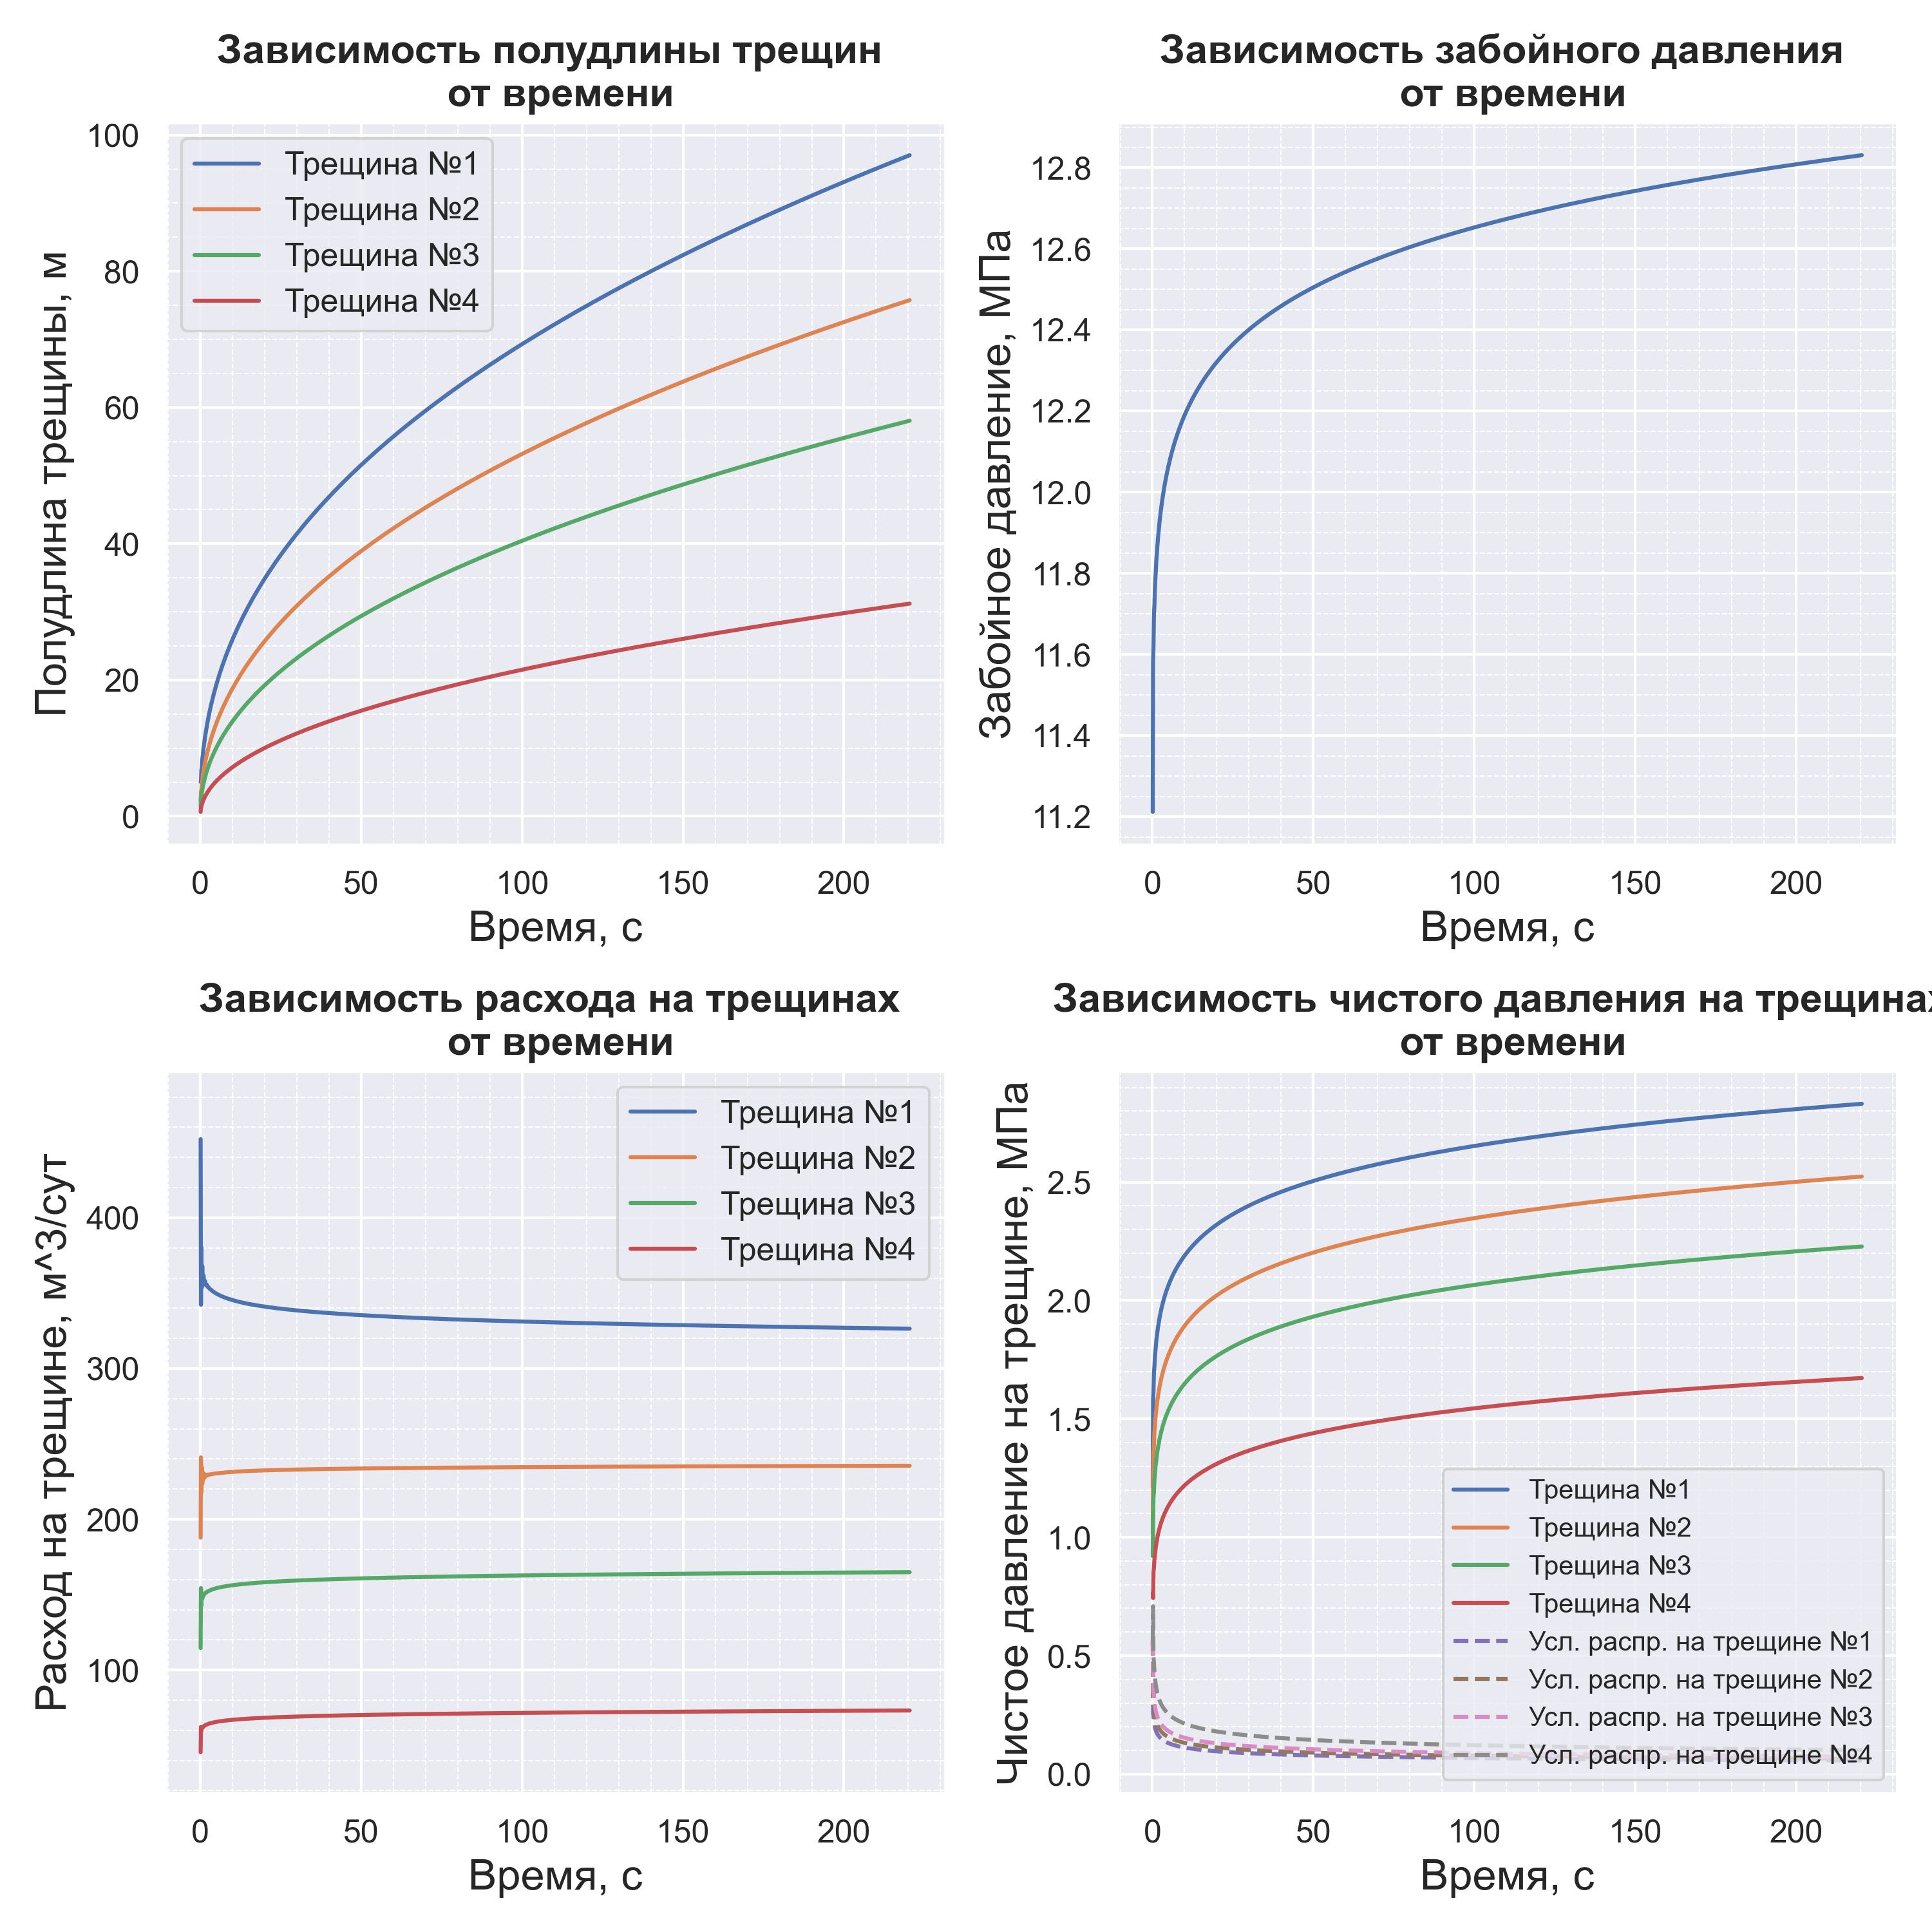
\includegraphics[width=8cm]{experiment_example1_300dpi.jpg}
\end{textblock*}

\begin{textblock*}{4cm}(8.8cm,3cm)
\footnotesize
Трещина 1 рассчитана с выбранными значениями входных параметров задачи.\\

На остальных трещинах ухудшены параметры перфораций.\\

$n_{p,2}=2;\,\,\,d_{p,2}=0.01\text{ м}$\\

$n_{p,3}=1;\,\,\,d_{p,3}=0.01\text{ м}$\\

$n_{p,4}=32;\,\,\,d_{p,4}=0.001\text{ м}$\\

\normalsize
\end{textblock*}

\end{frame}


\begin{frame}
\frametitle{Влияние резкого ухудшения качества перфораций на рост трещин}

\begin{textblock*}{8cm}(0.5cm,1.6cm)
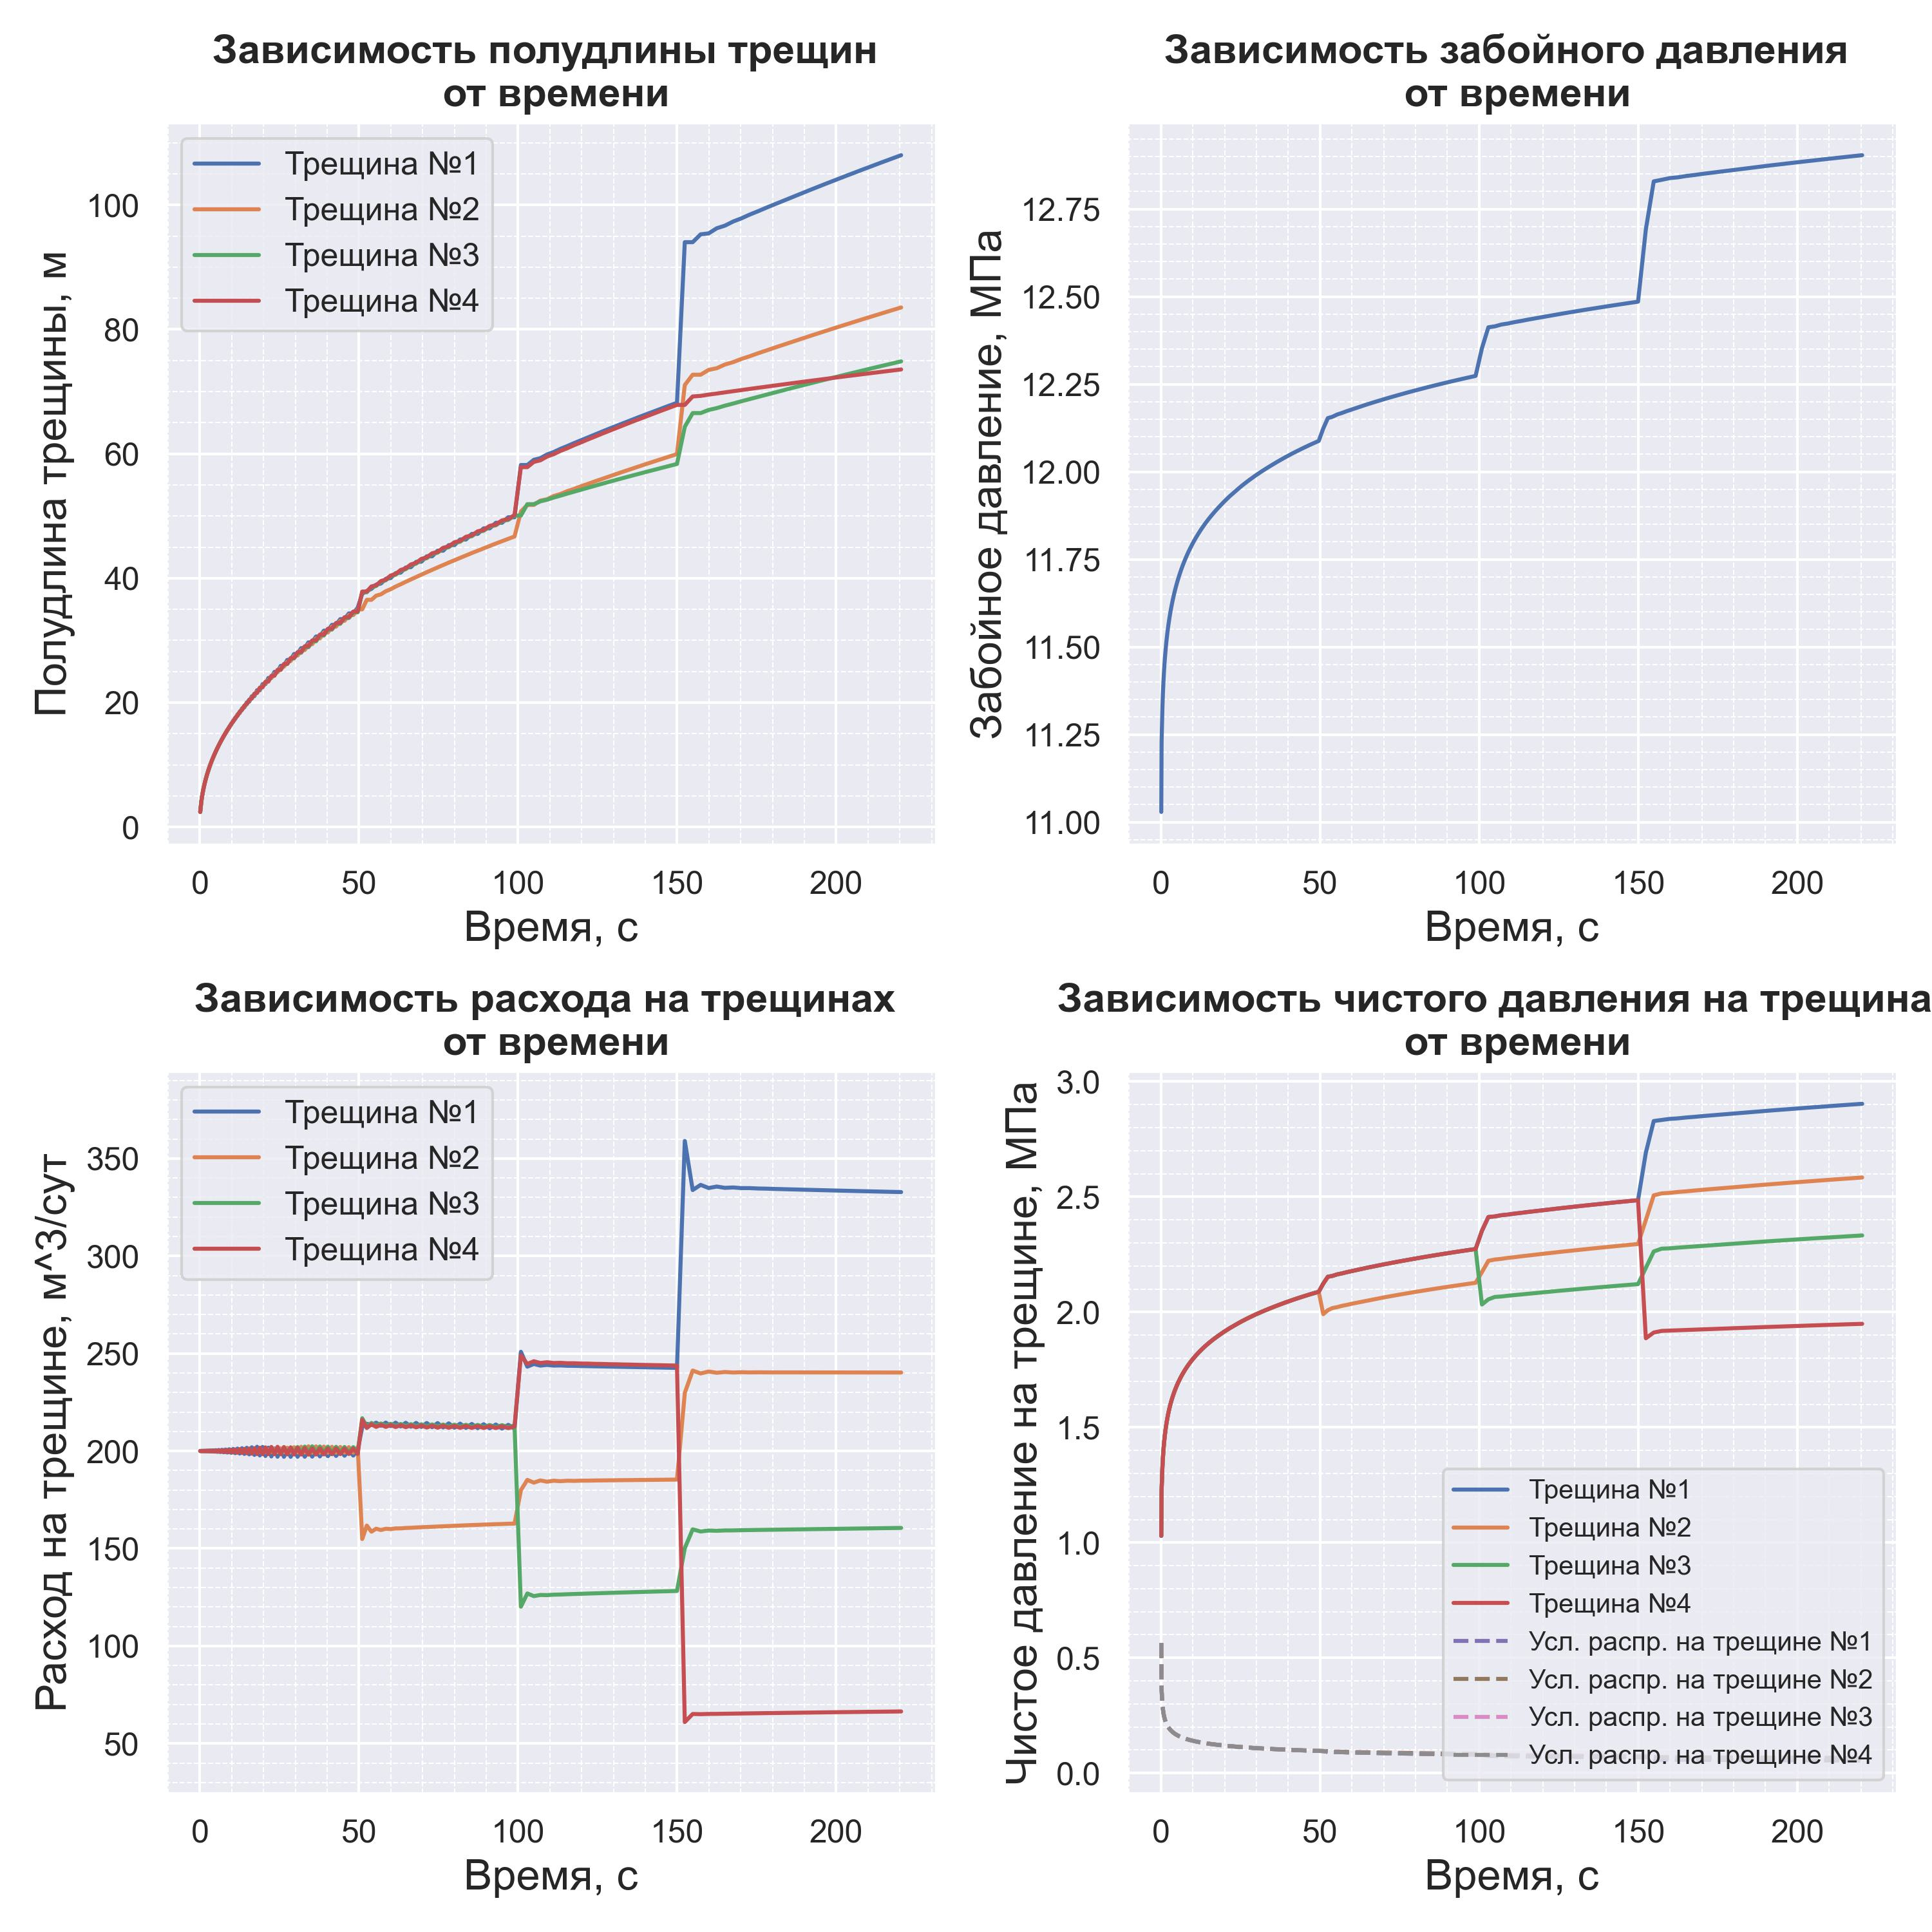
\includegraphics[width=8cm]{experiment_example2_300dpi.jpg}
\end{textblock*}

\begin{textblock*}{4cm}(8.8cm,1.5cm)
\footnotesize
Первые 50 секунд расчёт всех трещин проводился с выбранными значениями параметров задачи.\\

При $t=50\text{ с}$ ухудшено качество перфораций на второй трещине: $n_{p,2}=2;\,\,\,d_{p,2}=0.01\text{ м}$.\\

При $t=100\text{ с}$ ухудшено качество перфораций на третьей трещине: $n_{p,3}=1;\,\,\,d_{p,3}=0.01\text{ м}$.\\

При $t=150\text{ с}$ ухудшено качество перфораций на четвёртой трещине: $n_{p,4}=32;\,\,\,d_{p,4}=0.001\text{ м}$.\\

\normalsize
\end{textblock*}

\end{frame}


\begin{frame}
\frametitle{Выводы}

\small

\begin{itemize}
	\item Проведён обзор моделей трещины гидроразрыва пласта
	\item Реализован численный алгоритм расчёта потоков на каждой из трещин по законам Кирхгофа (при любом количестве трещин)
	\item Реализован алгоритм расчёта приращения полудлины трещины на каждом шаге по времени с учётом изменяющихся расходов и давления в трещинах (при любом количестве трещин)
	\item Сделан вывод, что внезапное ухудшение качества перфораций на одной из трещин может привести к неконтролируемому росту соседних трещин при фиксированном расходе на забое
\end{itemize}
\ \\

В дальнейшем необходимо дополнить построенную модель: учесть эффекты пороупругости, когда большие утечки из трещин влияют на упругое состояние породы и тем самым влияют на соседние трещины.
В этом случае может происходить эффект закрытия трещин автоГРП.

\normalsize

\end{frame}

\end{document}
